\chapter{Organic Molecules}
\label{chap:om}



% CHILD SECTION START 

\section{What is organic chemistry?}
\label{sec:om:hist}

\textbf{Organic chemistry} is the branch of chemistry that deals with \textbf{organic molecules}. An organic molecule is one which contains \textbf{carbon}, and these molecules can range in size from simple molecules to complex structures containing thousands of atoms! Although carbon is present in all organic compounds, other elements such as hydrogen (H), oxygen (O), nitrogen (N), sulfur (S) and phosphorus (P) are also common in these molecules.

Until the early nineteenth century, chemists had managed to make many simple compounds in the laboratory, but were still unable to produce the complex molecules that they found in living organisms. It was around this time that a Swedish chemist called \textbf{Jons Jakob Berzelius} suggested that compounds found only in living organisms (the organic compounds) should be grouped separately from those found in the non-living world (the inorganic compounds). He also suggested that the laws that governed how organic compounds formed, were different from those for inorganic compounds. From this, the idea developed that there was a 'vital force' in organic compounds. In other words, scientists believed that organic compounds would not follow the normal physical and chemical laws that applied to other inorganic compounds because the very 'force of life' made them different.

This idea of a mystical 'vital force' in organic compounds was weakened when scientists began to manufacture organic compounds in the laboratory from non-living materials. One of the first to do this was \textbf{Friedrich Wohler} in 1828, who successfully prepared urea, an organic compound in the urine of animals which, until that point, had only been found in animals. A few years later a student of Wohler's, \textbf{Hermann Kolbe}, made the organic compound \textit{acetic acid} from inorganic compounds. By this stage it was acknowledged that organic compounds are governed by exactly the same laws that apply to inorganic compounds. The properties of organic compounds are not due to a 'vital force' but to the unique properties of the carbon atom itself.\\

Organic compounds are very important in daily life. They make up a big part of our own bodies, they are in the food we eat and in the clothes we wear. Organic compounds are also used to make products such as medicines, plastics, washing powders, dyes, along with a list of other items. 


% CHILD SECTION END 



% CHILD SECTION START 

\section{Sources of carbon}
\label{sec:om:sources}

The main source of the carbon in organic compounds is \textbf{carbon dioxide} in the air. Plants use sunlight to convert carbon dioxide into organic compounds through the process of \textbf{photosynthesis}. Plants are therefore able to make their own organic compounds through photosynthesis, while animals feed on plants or plant products so that they gain the organic compounds that they need to survive. \\

Another important source of carbon is \textbf{fossil fuels} such as coal, petroleum and natural gas. This is because fossil fuels are themselves formed from the decaying remains of dead organisms (refer to Grade 11 for more information on fossil fuels). 


% CHILD SECTION END 



% CHILD SECTION START 

\section{Unique properties of carbon}
\label{sec:om:properties}

Carbon has a number of unique properties which influence how it behaves and how it bonds with other atoms:

\begin{itemize}
\item{Carbon has \textit{four valence electrons} which means that each carbon atom can form four bonds with other atoms. Because of this, long \textit{chain structures} can form. These chains can either be \textit{unbranched} (figure \ref{fig:organic:unbranched}) or \textit{branched} (figure \ref{fig:organic:branched}). Because of the number of bonds that carbon can form with other atoms, organic compounds can be very complex.
}

\begin{figure}[!h]
\begin{center}
\begin{pspicture}(-2,-1)(2,1)
%\psgrid[gridcolor=lightgray]
\rput(-1,0){\textbf{C}}
\rput(0,0){\textbf{C}}
\rput(1,0){\textbf{C}}
\rput(2,0){\textbf{C}}
\psline(-1.3,0)(-1.7,0)
\psline(-1,0.3)(-1,0.7)
\psline(-1,-0.3)(-1,-0.7)
\psline(-0.7,0)(-0.3,0)
\psline(0,0.3)(0,0.7)
\psline(0,-0.3)(0,-0.7)
\psline(0.3,0)(0.7,0)
\psline(1,0.3)(1,0.7)
\psline(1,-0.3)(1,-0.7)
\psline(1.3,0)(1.7,0)
\psline(2,0.3)(2,0.7)
\psline(2,-0.3)(2,-0.7)
\psline(2.3,0)(2.7,0)
\end{pspicture}
\end{center}
\caption{An unbranched carbon chain}
\label{fig:organic:unbranched}
\end{figure}

\begin{figure}[!h]
\begin{center}
\begin{pspicture}(-2,-4)(2,1)
%\psgrid[gridcolor=lightgray]
\rput(-1,0){\textbf{C}}
\rput(0,0){\textbf{C}}
\rput(1,0){\textbf{C}}
\rput(2,0){\textbf{C}}
\psline(-1.3,0)(-1.7,0)
\psline(-1,0.3)(-1,0.7)
\psline(-1,-0.3)(-1,-0.7)
\psline(-0.7,0)(-0.3,0)
\psline(0,0.3)(0,0.7)
\psline(0,-0.3)(0,-0.7)
\psline(0.3,0)(0.7,0)
\psline(1,0.3)(1,0.7)
\psline(1,-0.3)(1,-0.7)
\psline(1.3,0)(1.7,0)
\psline(2,0.3)(2,0.7)
\psline(2,-0.3)(2,-0.7)
\psline(2.3,0)(2.7,0)

\rput(0,-1){\textbf{C}}
\rput(0,-2){\textbf{C}}
\rput(0,-3){\textbf{C}}
\psline(-0.3,-1)(-0.7,-1)
\psline(0.3,-1)(0.7,-1)
\psline(0,-1.3)(0,-1.7)
\psline(-0.3,-2)(-0.7,-2)
\psline(0.3,-2)(0.7,-2)
\psline(0,-2.3)(0,-2.7)
\psline(-0.3,-3)(-0.7,-3)
\psline(0.3,-3)(0.7,-3)
\psline(0,-3.3)(0,-3.7)
\end{pspicture}
\end{center}
\caption{A branched carbon chain}
\label{fig:organic:branched}
\end{figure}

\item{Because of its position on the Periodic Table, most of the bonds that carbon forms with other atoms are \textit{covalent}. Think for example of a C-C bond. The difference in electronegativity between the two atoms is zero, so this is a pure covalent bond. In the case of a C-H bond, the difference in electronegativity between carbon (2.5) and hydrogen (2.1) is so small that C-H bonds are almost purely covalent. The result of this is that most organic compounds are non-polar. This affects some of the properties of organic compounds.}

\end{itemize}



% CHILD SECTION END 



% CHILD SECTION START 

\section{Representing organic compounds}
\label{sec:organic:representing}

There are a number of ways to represent organic compounds. It is useful to know all of these so that you can recognise a molecule however it is shown. There are three main ways of representing a compound. We will use the example of a molecule called 2-methylpropane to help explain the difference between each.

\subsection{Molecular formula}

The molecular formula of a compound shows how many atoms of each type are in a molecule. The number of each atom is written as a subscript after the atomic symbol. The molecular formula of 2-methylpropane is:

\begin{center}
\textbf{C$_{4}$H$_{10}$}
\end{center}


\subsection{Structural formula}

The structural formula of an organic compound shows every bond between every atom in the molecule. Each bond is represented by a line. The structural formula of 2-methylpropane is shown in figure \ref{fig:organic:structural formula}.

\begin{figure}[h]
\begin{center}
\begin{pspicture}(-3,-2)(4,4)
%\psgrid[gridcolor=lightgray]
\rput(-1,0){\textbf{C}}
\rput(0,0){\textbf{C}}
\rput(1,0){\textbf{C}}
\rput(-2.1,0){\textbf{H}}
\rput(-1,1.1){\textbf{H}}
\rput(-1,-1.1){\textbf{H}}
\rput(0,-1.1){\textbf{H}}
\rput(1,-1.1){\textbf{H}}
\psline(-1.3,0)(-1.7,0)
\psline(-1,0.3)(-1,0.7)
\psline(-1,-0.3)(-1,-0.7)
\psline(-0.7,0)(-0.3,0)
\psline(0,-0.3)(0,-0.7)
\psline(0.3,0)(0.7,0)
\psline(0,0.3)(0,1.7)
\psline(1,-0.3)(1,-0.7)
\psline(1.3,0)(1.7,0)
\rput(2,0){\textbf{H}}
\rput(0,2){\textbf{C}}
\psline(-0.3,2)(-0.7,2)
\rput(-1,2){\textbf{H}}
\psline(1,2)(1,2)
\rput(1,2){\textbf{H}}
\psline(0,2.3)(0,2.7)
\rput(0,3){\textbf{H}}
\psline(1,0.3)(1,0.7)
\rput(1,1){\textbf{H}}
\psline(0.3,2)(0.7,2)
\end{pspicture}
\caption{The structural formula of 2-methylpropane}
\label{fig:organic:structural formula}
\end{center}
\end{figure}

\subsection{Condensed structural formula}

When a compound is represented using its condensed structural formula, each carbon atom and the hydrogen atoms that are bonded directly to it are listed as a molecular formula, followed by a similar molecular formula for the neighbouring carbon atom. Branched groups are shown in brackets after the carbon atom to which they are bonded. The condensed structural formula below shows that in 2-methylpropane, there is a branched chain attached to the second carbon atom of the main chain. You can check this by looking at the structural formula in figure \ref{fig:organic:structural}. 

\begin{center}
\textbf{CH$_{3}$CH(CH$_{3}$)CH$_{3}$}
\end{center}

\Exercise{Representing organic compounds\\}{

\begin{enumerate}
\item{For each of the following organic compounds, give the \textbf{condensed structural formula} and the \textbf{molecular formula}.}
	\begin{enumerate}
	\item{
\begin{center}
\begin{pspicture}(-3,-2)(2,2)
%\psgrid[gridcolor=lightgray]
\rput(-1,0){\rput(-3,0){\textbf{H}}
\psline(-2.8,0)(-2.2,0)
\rput(-2,0){\textbf{C}}
\rput(-2,1){\textbf{H}}
\rput(-2,-1){\textbf{H}}
\psline(-2,0.2)(-2,0.8)
\psline(-2,-0.2)(-2,-0.8)
\psline(-1.8,0)(-1.2,0)
\rput(-1,0){\textbf{C}}
\psline(-1,0.2)(-1,0.8)
\rput(-1,1){\textbf{H}}
\psline(-0.8,0.05)(-0.2,0.05)
\psline(-0.8,-0.05)(-0.2, -0.05)
\rput(0,0){\textbf{C}}
\rput(0,1){\textbf{H}}
\psline(0,0.2)(0,0.8)
\psline(0.2,0)(0.8,0)
\rput(1,0){\textbf{C}}
\rput(1,1){\textbf{H}}
\rput(1,-1){\textbf{H}}
\psline(1,0.2)(1,0.8)
\psline(1,-0.2)(1,-0.8)
\rput(2,0){\textbf{H}}
\psline(1.2,0)(1.8,0)
}
\end{pspicture}
\end{center}}

	\item{
\begin{center}
\begin{pspicture}(-3,-1)(2.5,3.2)
%\psgrid[gridcolor=lightgray]
\rput(-1,0){\rput(-2,0){\textbf{C}}
\rput(-3,0.7){\textbf{H}}
\rput(-3,-0.7){\textbf{H}}
\psline(-2.2,0.2)(-2.8,0.5)
\psline(-2.2,-0.2)(-2.8,-0.5)
\psline(-1.8,0.05)(-1.2,0.05)
\psline(-1.8,-0.05)(-1.2,-0.05)
\rput(-1,0){\textbf{C}}
\rput(-1,1){\textbf{H}}
\psline(-1,0.2)(-1,0.8)
\psline(-0.2,0)(-0.8,0)
\rput(0,0){\textbf{C}}
\psline(0,-0.2)(0,-0.8)
\rput(0,-1){\textbf{H}}
\psline(0,0.2)(0,1.8)
\rput(0,2){\textbf{C}}
\psline(-0.2,2)(-0.8,2)
\rput(-1,2){\textbf{H}}
\psline(0,2.2)(0,2.8)
\rput(0,3){\textbf{H}}
\psline(0.2,2)(0.8,2)
\rput(1,2){\textbf{H}}
\psline(0.2,0)(0.8,0)
\rput(1,0){\textbf{C}}
\psline(1,0.2)(1,0.8)
\rput(1,1){\textbf{H}}
\psline(1,-0.2)(1,-0.8)
\rput(1,-1){\textbf{H}}
\psline(1.2,0)(1.8,0)
\rput(2,0){\textbf{H}}
}
\end{pspicture}
\end{center}}
	\end{enumerate}

\item{For each of the following, give the \textbf{structural formula} and the \textbf{molecular formula}.}
	\begin{enumerate}
	\item{CH$_{3}$CH$_{2}$CH$_{3}$}
	\item{CH$_{3}$CH$_{2}$CH(CH$_{3}$)CH$_{3}$}
	\item{C$_{2}$H$_{6}$}
	\end{enumerate}

\item{Give two possible structural formulae for the compound with a molecular formula of C$_{4}$H$_{10}$.}
\end{enumerate}
}


% CHILD SECTION END 



% CHILD SECTION START 

\section{Isomerism in organic compounds}
\label{sec:organic:isomer}

It is possible for two organic compounds to have the same \textit{molecular formula} but a different \textit{structural formula}. Look for example at the two organic compounds that are shown in figure \ref{fig:organic:butane}.

\begin{figure}[h]
\begin{center}
 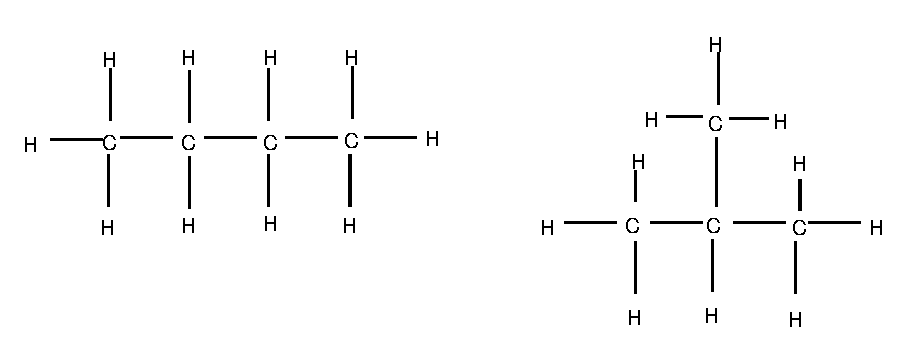
\includegraphics{../../epsimages/isomer_butane.eps}
 % isomer_butane.eps: 0x0 pixel, 300dpi, 0.00x0.00 cm, bb=5 2 427 155
\end{center}


% \begin{pspicture}(-3,-1.5)(4,3)
% %\psgrid[gridcolor=lightgray]
% \rput(-3,0){
% \rput(-1,0){\textbf{C}}
% \rput(0,0){\textbf{C}}
% \rput(1,0){\textbf{C}}
% \rput(2,0){\textbf{C}}
% \rput(-2.1,0){\textbf{H}}
% \rput(-1,1.1){\textbf{H}}
% \rput(-1,-1.1){\textbf{H}}
% \rput(0,1.1){\textbf{H}}
% \rput(0,-1.1){\textbf{H}}
% \rput(1,1.1){\textbf{H}}
% \rput(1,-1.1){\textbf{H}}
% \rput(2,1.1){\textbf{H}}
% \rput(2,-1.1){\textbf{H}}
% \rput(3,0){\textbf{H}}
% \psline(-1.3,0)(-1.7,0)
% \psline(-1,0.3)(-1,0.7)
% \psline(-1,-0.3)(-1,-0.7)
% \psline(-0.7,0)(-0.3,0)
% \psline(0,0.3)(0,0.7)
% \psline(0,-0.3)(0,-0.7)
% \psline(0.3,0)(0.7,0)
% \psline(1,0.3)(1,0.7)
% \psline(1,-0.3)(1,-0.7)
% \psline(1.3,0)(1.7,0)
% \psline(2,0.3)(2,0.7)
% \psline(2,-0.3)(2,-0.7)
% \psline(2.3,0)(2.7,0)
% \rput(6.5,0){
% \rput(-1,0){\textbf{C}}
% \rput(0,0){\textbf{C}}
% \rput(1,0){\textbf{C}}
% \rput(-2.1,0){\textbf{H}}
% \rput(-1,1.1){\textbf{H}}
% \rput(-1,-1.1){\textbf{H}}
% \rput(0,1.1){\textbf{H}}
% \rput(0,-1.1){\textbf{H}}
% \rput(1,-1.1){\textbf{H}}
% \psline(-1.3,0)(-1.7,0)
% \psline(-1,0.3)(-1,0.7)
% \psline(-1,-0.3)(-1,-0.7)
% \psline(-0.7,0)(-0.3,0)
% \psline(0,0.3)(0,0.7)
% \psline(0,-0.3)(0,-0.7)
% \psline(0.3,0)(0.7,0)
% \psline(1,0.3)(1,1.7)
% \psline(1,-0.3)(1,-0.7)
% \psline(1.3,0)(1.7,0)
% \rput(2,0){\textbf{H}}
% \rput(1,2){\textbf{C}}
% \psline(0.7,2)(0.3,2)
% \rput(0,2){\textbf{H}}
% \psline(1.3,2)(1.7,2)
% \rput(2,2){\textbf{H}}
% \psline(1,2.3)(1,2.7)
% \rput(1,3){\textbf{H}}
% }
% }
% \end{pspicture}
% \end{center}
\caption{Isomers of a 4-carbon organic compound}
\label{fig:organic:butane}
\end{figure}

If you were to count the number of carbon and hydrogen atoms in each compound, you would find that they are the same. They both have the same molecular formula (C$_{4}$H$_{10}$), but their structure is different and so are their properties. Such compounds are called \textbf{isomers}.

\Definition{Isomer}{
In chemistry, isomers are molecules with the same molecular formula and often with the same kinds of chemical bonds between atoms, but in which the atoms are arranged differently.
}

\Exercise{Isomers\\}{

Match the organic compound in Column A with its isomer Column B:\\

\begin{center}
\begin{tabular}{|c|c|}\hline
\textbf{Column A} & \textbf{Column B}\\\hline
CH$_{3}$CH(CH$_{3}$)OH & CH$_{3}$CH(CH$_{3}$)CH$_{3}$ \\\hline

\begin{pspicture}(0,-1.3)(5,1.3)
\rput(0,0){H}

\psline(0.3,0)(0.7,0)
\rput(1,0){C}
\psline(1,0.3)(1,0.7)
\rput(1,1){H}
\psline(1,-0.3)(1,-0.7)
\rput(1,-1){H}
\rput(1,0){
\psline(0.3,0)(0.7,0)
\rput(1,0){C}
\psline(1,0.3)(1,0.7)
\rput(1,1){H}
\psline(1,-0.3)(1,-0.7)
\rput(1,-1){H}
}
\rput(2,0){
\psline(0.3,0)(0.7,0)
\rput(1,0){C}
\psline(1,0.3)(1,0.7)
\rput(1,1){H}
\psline(1,-0.3)(1,-0.7)
\rput(1,-1){H}
}
\rput(3,0){
\psline(0.3,0)(0.7,0)
\rput(1,0){C}
\psline(1,0.3)(1,0.7)
\rput(1,1){H}
\psline(1,-0.3)(1,-0.7)
\rput(1,-1){H}
}
\psline(4.3,0)(4.7,0)
\rput(5,0){H}
\end{pspicture}

&

\begin{pspicture}(0,-1.3)(5,1.3)
\rput(0,0){H}

\psline(0.3,0)(0.7,0)
\rput(1,0){C}
\psline(1,0.3)(1,0.7)
\rput(1,1){H}
\psline(1,-0.3)(1,-0.7)
\rput(1,-1){H}
\rput(1,0){
\psline(0.3,0)(0.7,0)
\rput(1,0){C}
\psline(1,0.3)(1,0.7)
\rput(1,1){H}
\psline(1,-0.3)(1,-0.7)
\rput(1,-1){H}
}
\rput(2,0){
\psline(0.3,0)(0.7,0)
\rput(1,0){C}
\psline(1,0.3)(1,0.7)
\rput(1,1){CH$_{3}$}
\psline(1,-0.3)(1,-0.7)
\rput(1,-1){H}
}
\psline(3.3,0)(3.7,0)
\rput(4,0){H}
\end{pspicture}\\\hline

\begin{pspicture}(0,-1.3)(5,1.3)
\rput(0,0){H}

\psline(0.3,0)(0.7,0)
\rput(1,0){C}
\psline(1,0.3)(1,0.7)
\rput(1,1){CH$_{3}$}
\psline(1,-0.3)(1,-0.7)
\rput(1,-1){H}
\rput(1,0){
\psline(0.3,0)(0.7,0)
\rput(1,0){C}
\psline(1,0.3)(1,0.7)
\rput(1,1){H}
\psline(1,-0.3)(1,-0.7)
\rput(1,-1){H}
}
\rput(2,0){
\psline(0.3,0)(0.7,0)
\rput(1,0){C}
\psline(1,0.3)(1,0.7)
\rput(1,1){H}
\psline(1,-0.3)(1,-0.7)
\rput(1,-1){H}
}
\psline(3.3,0)(3.7,0)
\rput(4,0){H}
\end{pspicture}

& 

C$_{3}$H$_{7}$OH \\\hline

\end{tabular}
\end{center}
}



% CHILD SECTION END 



% CHILD SECTION START 

\section{Functional groups}
\label{sec:organic:functional}

All organic compounds have a particular bond or group of atoms which we call its \textbf{functional group}. This group is important in determining how a compound will react. 

\Definition{Functional group}{
In organic chemistry, a functional group is a specific group of atoms within molecules, that are responsible for the characteristic chemical reactions of those molecules. The same functional group will undergo the same or similar chemical reaction(s) regardless of the size of the molecule it is a part of.
}

In one group of organic compounds called the \textbf{hydrocarbons}, the single, double and triple bonds of the alkanes, alkenes and alkynes are examples of functional groups. In another group, the alcohols, an oxygen and a hydrogen atom   are bonded to each other to form the functional group for those compounds (in other words an alcohol has an OH in it). All alcohols will contain an oxygen and a hydrogen atom bonded together in some part of the molecule. \\

Table \ref{fig:om:summary} summarises some of the common functional groups. We will look at these in more detail later in this chapter.

\begin{table}[!h]
\begin{center}
\begin{tabular}{|l|c|c|c|}\hline
\textbf{Name of group} & \textbf{Functional group} & \textbf{Example} & \textbf{Diagram}\\\hline
Alk\textit{ane} & 
\begin{pspicture}(-2,-1.5)(1,1.5)
%\psgrid[gridcolor=lightgray]
\rput(-1,0){C} \rput(0,0){C} \psline(-0.8,0)(-0.2,0) \psline(0.2,0)(0.8,0)
\psline(-1.2,0)(-1.8,0)
\psline(-1,0.2)(-1,0.8)
\psline(-1,-0.2)(-1,-0.8)
\psline(0,0.2)(0,0.8)
\psline(0,-0.2)(0,-0.8)
\end{pspicture}
& Ethane &
\begin{pspicture}(-2,-1.5)(1,1.5)
%\psgrid[gridcolor=lightgray]
\rput(-1,0){C}
\rput(0,0){C}
\psline(-0.8,0)(-0.2,0)
\psline(0.2,0)(0.8,0)
\psline(-1.2,0)(-1.8,0)
\psline(-1,0.2)(-1,0.8)
\psline(-1,-0.2)(-1,-0.8)
\psline(0,0.2)(0,0.8)
\psline(0,-0.2)(0,-0.8)
\rput(-2,0){H}
\rput(1,0){H}
\rput(-1,1){H}
\rput(-1,-1){H}
\rput(0,1){H}
\rput(0,-1){H}
\end{pspicture}
\\\hline

Alk\textit{ene} & 
\begin{pspicture}(-2,-1.5)(1,1.5)
%\psgrid[gridcolor=lightgray]
\rput(-1,0){\textbf{C}}

\rput(0,0){\textbf{C}}
\psline(-0.8,-0.05)(-0.2,-0.05)
\psline(-0.8,0.05)(-0.2,0.05)
\psline(0.2,0.2)(0.7,0.7)
\psline(0.2,-0.2)(0.7,-0.7)
\psline(-1.2,0.2)(-1.7,0.7)
\psline(-1.2,-0.2)(-1.7,-0.7)
\end{pspicture} & Ethene & 

\begin{pspicture}(-2,-1.5)(1,1.5)
%\psgrid[gridcolor=lightgray]
\rput(-1,0){\textbf{C}}
\rput(0,0){\textbf{C}}
\psline(-0.8,-0.05)(-0.2,-0.05)
\psline(-0.8,0.05)(-0.2,0.05)
\psline(0.2,0.2)(0.7,0.7)
\psline(0.2,-0.2)(0.7,-0.7)
\psline(-1.2,0.2)(-1.7,0.7)
\psline(-1.2,-0.2)(-1.7,-0.7)
\rput(1,1){\textbf{H}}
\rput(1,-1){\textbf{H}}
\rput(-2,1){\textbf{H}}
\rput(-2,-1){\textbf{H}}
\end{pspicture}
\\\hline

Alk\textit{yne} & 
\begin{pspicture}(-2,-1)(1,1)
%\psgrid[gridcolor=lightgray]
\rput(-1,0){\textbf{C}}
\rput(0,0){\textbf{C}}
\psline(-1.8,0)(-1.2,0)
\psline(-0.8,0.075)(-0.2,0.075)
\psline(-0.8,0)(-0.2,0)
\psline(-0.8,-0.075)(-0.2,-0.075)
\psline(0.2,0)(0.8,0)
\end{pspicture} &
Ethyne (acetylene) & 

\begin{pspicture}(-2,-1)(1,1)
%\psgrid[gridcolor=lightgray]
\rput(-2,0){\textbf{H}}
\rput(-1,0){\textbf{C}}
\rput(0,0){\textbf{C}}
\rput(1,0){\textbf{H}}
\psline(-1.8,0)(-1.2,0)
\psline(-0.8,0.075)(-0.2,0.075)
\psline(-0.8,0)(-0.2,0)
\psline(-0.8,-0.075)(-0.2,-0.075)
\psline(0.2,0)(0.8,0)
\end{pspicture}
\\\hline

Halo-alkane & 
\begin{pspicture}(-2,-2)(0,1)
\rput(-1,0){\textbf{C}}
\rput(0,0){\textbf{X}}
\rput(-1,-1.5){(X=F,Cl,Br,I)}
\psline(-1.2,0)(-1.8,0)
\psline(-0.2,0)(-0.8,0)
\psline(-1,0.2)(-1,0.8)
\psline(-1,-0.2)(-1,-0.8)
\end{pspicture} & Chloroethane & 

\begin{pspicture}(-2,-2)(0,1.5)
\rput(-1,0){\textbf{C}}
\rput(-2.2,0){\textbf{CH$_{3}$}}
\rput(0,0){\textbf{X}}
\psline(-1.2,0)(-1.8,0)
\psline(-0.2,0)(-0.8,0)
\psline(-1,0.2)(-1,0.8)
\psline(-1,-0.2)(-1,-0.8)
\rput(-1,1){\textbf{H}}
\rput(-1,-1){\textbf{H}}
\end{pspicture}\\\hline

Alcoh\textit{ol}/ alkan\textit{ol} & 
\begin{pspicture}(-2,-2)(0,1)
\rput(-1,0){\textbf{C}}
\rput(0,0){\textbf{OH}}
\psline(-1.2,0)(-1.8,0)
\psline(-0.2,0)(-0.8,0)
\psline(-1,0.2)(-1,0.8)
\psline(-1,-0.2)(-1,-0.8)
\end{pspicture} & Ethanol & 

\begin{pspicture}(0,-1.5)(3,1.5)
\rput(0,0){\textbf{H}}
\rput(1,0){\textbf{C}}
\rput(2,0){\textbf{C}}
\rput(3,0){\textbf{H}}
\rput(1,1){\textbf{H}}
\rput(1,-1){\textbf{H}}
\rput(2,1){\textbf{OH}}
\rput(2,-1){\textbf{H}}
\rput(3,0){\textbf{H}}
\psline(0.2,0)(0.8,0)
\psline(1.2,0)(1.8,0)
\psline(2.2,0)(2.8,0)
\psline(1,0.2)(1,0.8)
\psline(1,-0.2)(1,-0.8)
\psline(2,0.2)(2,0.8)
\psline(2,-0.2)(2,-0.8)
\end{pspicture}\\\hline

Carboxylic acid & 
\begin{pspicture}(-1,-1)(1,1)
\rput(0,0){\textbf{C}}
\rput(0.6,0.6){\textbf{O}}
\rput(0.6,-0.6){\textbf{OH}}
\psline(-0.2,0)(-0.8,0)
\psline(0.05,0.2)(0.5,0.5)
\psline(-0.05,0.2)(0.4,0.5)
\psline(0,-0.2)(0.6,-0.5) 
\end{pspicture} & ethanoic acid & 

\begin{pspicture}(-2,-1)(2,1.5)
\rput(-1.7,0){\textbf{CH$_{3}$}}
\psline(-1.2,0)(-0.6,0)
\rput(-0.4,0){\textbf{C}}
\rput(-0.4,1){\textbf{O}}
\psline(-0.35,0.2)(-0.35,0.8)
\psline(-0.45,0.2)(-0.45,0.8)
\psline(-0.2,0)(0.4,0)
\rput(0.8,0){\textbf{OH}}
\end{pspicture}\\\hline

Amine & 
\begin{pspicture}(-2.5,-1)(1,1.5)
\rput(-1,0){\textbf{N}}
\rput(-2,0){\textbf{R}}
\rput(0,0.8){\textbf{H}}
\rput(0,-0.8){\textbf{H}}
\psline(-1.2,0)(-1.8,0)
\psline(-0.8,0.2)(-0.2,0.6)
\psline(-0.8,-0.2)(-0.2,-0.6)
\end{pspicture} & Glycine &

\begin{pspicture}(-2.5,-2)(2.5,2)
\rput(0,0){\textbf{C}}
\rput(0,1){\textbf{H}}
\rput(0,-1){\textbf{H}}
\rput(1,0){\textbf{N}}
\rput(2,0.8){\textbf{H}}
\rput(2,-0.8){\textbf{H}}
\rput(-1,0){\textbf{C}}
\rput(-2,0.8){\textbf{O}}
\rput(-2,-0.8){\textbf{OH}}
\psline(0,0.2)(0,0.8)
\psline(0,-0.2)(0,-0.8)
\psline(-0.2,0)(-0.8,0)
\psline(-1.15,0.2)(-1.75,0.6)
\psline(-1.25,0.2)(-1.85,0.6)
\psline(-1.2,-0.2)(-1.8,-0.6)
\psline(0.2,0)(0.8,0)
\psline(1.2,0.2)(1.8,0.6)
\psline(1.2,-0.2)(1.8,-0.6)
\end{pspicture}\\\hline

\end{tabular}
\end{center}
\caption{Some functional groups of organic compounds}
\label{fig:om:summary}
\end{table}



% CHILD SECTION END 



% CHILD SECTION START 

\section{The Hydrocarbons}
\label{sec:organic:hydrocarbons}

Let us first look at a group of organic compounds known as the \textbf{hydrocarbons}. These molecules only contain carbon and hydrogen. The hydrocarbons that we are going to look at are called \textbf{aliphatic compounds}. The aliphatic compounds are divided into \textit{acyclic compounds} (chain structures) and \textit{cyclic compounds} (ring structures). The chain structures are further divided into structures that contain only \textit{single bonds} (\textbf{alkanes}), those that contain at least one \textit{double bond} (\textbf{alkenes}) and those that contain at least one \textit{triple bond} (\textbf{alkynes}). Cyclic compounds include structures such as the \textit{benzene ring}. Figure \ref{fig:om:classhydro} summarises the classification of the hydrocarbons. \\

\begin{figure}[h]
\begin{center}
\begin{pspicture}(-8,0)(8,5)
%\psgrid[gridcolor=lightgray]
\rput(0,4){Aliphatic hydrocarbons}
\psline(0,3.8)(0,3.2)
\psline(-6,3.2)(6,3.2)
\psline(-6,3.2)(-6,2.6)
\psline(6,3.2)(6,2.6)
\rput(-6,2.5){Acyclic compounds}
\rput(-6,2.2){(chain structures)}
\rput(6,2.5){Cyclic compounds}
\rput(6,2.2){(ring structures e.g. benzene ring)}
\psline(-6,2)(-6,1.4)
\psline(-7,1.4)(4,1.4)
\psline(-7,1.4)(-7,0.8)
\psline(-2,1.4)(-2,0.8)
\psline(4,1.4)(4,0.8)
\rput(-7,0.3){Alkanes (single bonds)}
\rput(-2,0.3){Alkenes (contain double bonds)}
\rput(4,0.3){Alkynes (contain triple bonds)}
\end{pspicture}
\end{center}
\caption{The classification of the aliphatic hydrocarbons}
\label{fig:om:classhydro}
\end{figure}

Hydrocarbons that contain only single bonds are called \textbf{saturated} hydrocarbons because each carbon atom is bonded to as many hydrogen atoms as possible. Figure \ref{fig:organic:saturated} shows a molecule of ethane which is a saturated hydrocarbon.\\

\begin{figure}[!h]
\begin{center}
\begin{pspicture}(-2,-1)(1,2)
%\psgrid[gridcolor=lightgray]
\rput(-1,0){C}
\rput(0,0){C}
\psline(-0.8,0)(-0.2,0)
\psline(0.2,0)(0.8,0)
\psline(-1.2,0)(-1.8,0)
\psline(-1,0.2)(-1,0.8)
\psline(-1,-0.2)(-1,-0.8)
\psline(0,0.2)(0,0.8)
\psline(0,-0.2)(0,-0.8)
\rput(-2,0){H}
\rput(1,0){H}
\rput(-1,1){H}
\rput(-1,-1){H}
\rput(0,1){H}
\rput(0,-1){H}
\end{pspicture}
\end{center}
\caption{A saturated hydrocarbon}
\label{fig:organic:saturated}
\end{figure}

Hydrocarbons that contain double or triple bonds are called \textbf{unsaturated} hydrocarbons because they don't contain as many hydrogen atoms as possible. Figure \ref{fig:organic:unsaturated} shows a molecule of ethene which is an unsaturated hydrocarbon. If you compare the number of carbon and hydrogen atoms in a molecule of ethane and a molecule of ethene, you will see that the number of hydrogen atoms in ethene is \textit{less} than the number of hydrogen atoms in ethane despite the fact that they both contain two carbon atoms. In order for an unsaturated compound to become saturated, a double bond has to be broken, and another two hydrogen atoms added for each double bond that is replaced by a single bond.

\begin{figure}[!h]
\begin{center}
\begin{pspicture}(-2,-1)(1,2)
%\psgrid[gridcolor=lightgray]
\rput(-1,0){\textbf{C}}
\rput(0,0){\textbf{C}}
\psline(-0.8,-0.05)(-0.2,-0.05)
\psline(-0.8,0.05)(-0.2,0.05)
\psline(0.2,0.2)(0.7,0.7)
\psline(0.2,-0.2)(0.7,-0.7)
\psline(-1.2,0.2)(-1.7,0.7)
\psline(-1.2,-0.2)(-1.7,-0.7)
\rput(1,1){\textbf{H}}
\rput(1,-1){\textbf{H}}
\rput(-2,1){\textbf{H}}
\rput(-2,-1){\textbf{H}}
\end{pspicture}
\end{center}
\caption{An unsaturated hydrocarbon}
\label{fig:organic:unsaturated}
\end{figure}

\begin{IFact}{
Fat that occurs naturally in living matter such as animals and plants is used as food for human consumption and contains varying proportions of saturated and unsaturated fat. Foods that contain a high proportion of saturated fat are butter, ghee, suet, tallow, lard, coconut oil, cottonseed oil, and palm kernel oil, dairy products (especially cream and cheese), meat, and some prepared foods. Diets high in saturated fat are correlated with an increased incidence of atherosclerosis and coronary heart disease according to a number of studies. Vegetable oils contain unsaturated fats and can be hardened to form margarine by adding hydrogen on to some of the carbon=carbon double bonds using a nickel catalyst. The process is called hydrogenation
}
\end{IFact}

We will now go on to look at each of the hydrocarbon groups in more detail. These groups are the alkanes, the alkenes and the alkynes.

\subsection{The Alkanes}

The alkanes are hydrocarbons that only contain \textit{single covalent bonds} between their carbon atoms. This means that they are \textit{saturated} compounds and are quite unreactive. The simplest alkane has only one carbon atom and is called \textbf{methane}. This molecule is shown in figure \ref{fig:organic:methane}.

\begin{figure}[!h]
\begin{center}
\begin{pspicture}(-3,-1)(3,1.5)
%\psgrid[gridcolor=lightgray]
\rput(-1,0){\textbf{C}}
\rput(-2,0){\textbf{H}}
\rput(0,0){\textbf{H}}
\rput(-1,1){\textbf{H}}
\rput(-1,-1){\textbf{H}}
\psline(-0.2,0)(-0.8,0)
\psline(-1.2,0)(-1.8,0)
\psline(-1,0.2)(-1,0.8)
\psline(-1,-0.2)(-1,-0.8)
\rput(-2.8,0){\textbf{(a)}}
\rput(1,0){\textbf{(b)}}
\rput(2,0){\textbf{CH$_{4}$}}
\end{pspicture}
\end{center}
\caption{The structural (a) and molecular formula (b) for methane}
\label{fig:organic:methane}
\end{figure}

The second alkane in the series has two carbon atoms and is called \textbf{ethane}. This is shown in figure \ref{fig:organic:ethane}.\\

\begin{figure}[!h]
\begin{center}
\begin{pspicture}(-3,-1)(5,1.5)
%\psgrid[gridcolor=lightgray]
\rput(-1,0){\textbf{C}}
\rput(-2,0){\textbf{H}}
\rput(-1,1){\textbf{H}}
\rput(-1,-1){\textbf{H}}
\rput(0,0){\textbf{C}}
\rput(1,0){\textbf{H}}
\rput(0,1){\textbf{H}}
\rput(0,-1){\textbf{H}}
\psline(-0.2,0)(-0.8,0)
\psline(-1.2,0)(-1.8,0)
\psline(-1,0.2)(-1,0.8)
\psline(-1,-0.2)(-1,-0.8)
\psline(0.2,0)(0.8,0)
\psline(0,0.2)(0,0.8)
\psline(0,-0.2)(0,-0.8)
\rput(-2.8,0){\textbf{(a)}}
\rput(3,0){\textbf{(b)}}
\rput(4,0){\textbf{C$_{2}$H$_{6}$}}
\end{pspicture}
\end{center}
\caption{The structural (a) and molecular formula (b) for ethane}
\label{fig:organic:ethane}
\end{figure}

The third alkane in the series has three carbon atoms and is called \textbf{propane} (Figure \ref{fig:organic:propane}).

\begin{figure}[!h]
\begin{center}
\begin{pspicture}(-3,-1)(5,1.5)
%\psgrid[gridcolor=lightgray]
\rput(-1,0){\textbf{C}}
\rput(-2,0){\textbf{H}}
\rput(-1,1){\textbf{H}}
\rput(-1,-1){\textbf{H}}
\rput(0,0){\textbf{C}}
\rput(0,1){\textbf{H}}
\rput(0,-1){\textbf{H}}
\rput(1,0){\textbf{C}}
\rput(2,0){\textbf{H}}
\rput(1,1){\textbf{H}}
\rput(1,-1){\textbf{H}}
\psline(-0.2,0)(-0.8,0)
\psline(-1.2,0)(-1.8,0)
\psline(-1,0.2)(-1,0.8)
\psline(-1,-0.2)(-1,-0.8)
\psline(0.2,0)(0.8,0)
\psline(0,0.2)(0,0.8)
\psline(0,-0.2)(0,-0.8)
\psline(1.2,0)(1.8,0)
\psline(1,0.2)(1,0.8)
\psline(1,-0.2)(1,-0.8)
\rput(-2.8,0){\textbf{(a)}}
\rput(3,0){\textbf{(b)}}
\rput(4,0){\textbf{C$_{3}$H$_{8}$}}
\end{pspicture}
\end{center}
\caption{The structural (a) and molecular formula (b) for propane}
\label{fig:organic:propane}
\end{figure}

When you look at the molecular formula for each of the alkanes, you should notice a pattern developing. For each carbon atom that is added to the molecule, two hydrogen atoms are added. In other words, each molecule differs from the one before it by CH$_{2}$. This is called a \textit{homologous series}. The alkanes have the general formula C$_{n}$H$_{2n+2}$.

The alkanes are the most important source of fuel in the world and are used extensively in the chemical industry. Some are gases (e.g. methane and ethane), while others are liquid fuels (e.g. octane, an important component of petrol).

\begin{IFact}{Some fungi use alkanes as a source of carbon and energy. One fungus \textit{Amorphotheca resinae} prefers the alkanes used in aviation fuel, and this can cause problems for aircraft in tropical areas!}
\end{IFact}

\subsection{Naming the alkanes}

In order to give compounds a name, certain rules must be followed. When naming organic compounds, the IUPAC (International Union of Pure and Applied Chemistry) nomenclature is used. We will first look at some of the steps that need to be followed when naming a compound, and then try to apply these rules to some specific examples.

\begin{enumerate}
\item{STEP 1: Recognise the \textit{functional group} in the compound. This will determine the suffix (the 'end') of the name. For example, if the compound is an alkane, the suffix will be -ane; if the compound is an alkene the suffix will be -ene; if the compound is an alcohol the suffix will be -ol, and so on.}
\item{STEP 2: Find the longest continuous carbon chain (it won't always be a \textit{straight} chain) and count the number of carbon atoms in this chain. This number will determine the prefix (the 'beginning') of the compound's name. These prefixes are shown in table \ref{tab:prefix}. So, for example, an alkane that has 3 carbon atoms will have the suffix \textit{prop} and the compound's name will be \textit{propane}.

\begin{table}[!h]
\begin{center}
\begin{tabular}{|c|c|}\hline
\textbf{Carbon atoms} & prefix \\\hline

1 & meth(ane)\\\hline
2 & eth(ane)\\\hline
3 & prop(ane)\\\hline
4 & but(ane) \\\hline
5 & pent(ane) \\\hline
6 & hex(ane) \\\hline
7 & hept(ane) \\\hline
8 & oct(ane) \\\hline
9 & non(ane) \\\hline
10 & dec(ane) \\\hline
\end{tabular}
\end{center}
\caption{The prefix of a compound's name is determined by the number of carbon atoms in the longest chain}
\label{tab:prefix}
\end{table}
}
\item{STEP 3: Number the carbons in the longest carbon chain (Important: If there is a double or triple bond, you need to start numbering so that the bond is at the carbon with the lowest number.}
\item{STEP 4: Look for any branched groups and name them. Also give them a number to show their position on the carbon chain. If there are no branched groups, this step can be left out.}
\item{STEP 5: Combine the elements of the name into a single word in the following order: branched groups; prefix; name ending according to the functional group and its position along the longest carbon chain.}
\end{enumerate}
Khan Academy video on naming simple alkanes: SIYAVULA-VIDEO:http://cnx.org/content/m39453/latest/#alkanes-1
\begin{wex}{Naming the alkanes}{Give the IUPAC name for the following compound:
\begin{figure}[H]
\begin{center}
\begin{pspicture}(-3,-1.5)(4,1.5)
%\psgrid[gridcolor=lightgray]
\rput(-1,0){\textbf{C$_{(1)}$}}
\rput(-2,0){\textbf{H}}
\rput(-1,1){\textbf{H}}
\rput(-1,-1){\textbf{H}}
\rput(0,0){\textbf{C$_{(2)}$}}
\rput(0,1){\textbf{H}}
\rput(0,-1){\textbf{H}}
\rput(1,0){\textbf{C$_{(3)}$}}
\rput(2,0){\textbf{C$_{(4)}$}}
\rput(1,1){\textbf{H}}
\rput(1,-1){\textbf{H}}
\psline(-0.2,0)(-0.8,0)
\psline(-1.2,0)(-1.8,0)
\psline(-1,0.2)(-1,0.8)
\psline(-1,-0.2)(-1,-0.8)
\psline(0.2,0)(0.8,0)
\psline(0,0.2)(0,0.8)
\psline(0,-0.2)(0,-0.8)
\psline(1.2,0)(1.8,0)
\psline(1,0.2)(1,0.8)
\psline(1,-0.2)(1,-0.8)
\rput(2,1){\textbf{H}}
\rput(2,-1){\textbf{H}}
\rput(3,0){\textbf{H}}
\psline(2.2,0)(2.8,0)
\psline(2,0.2)(2,0.8)
\psline(2,-0.2)(2,-0.8)
\end{pspicture}
\end{center}
\end{figure}
Note: The numbers attached to the carbon atoms would not normally be shown. The atoms have been numbered to help you to name the compound.
}
{\westep{Identify the functional group}
The compound is a hydrocarbon with single bonds between the carbon atoms. It is an alkane and will have a suffix of -ane.

\westep{Find the longest carbon chain}
There are four carbon atoms in the longest chain. The prefix of the compound will be 'but'.
\westep{Number the carbons in the longest chain}
In this case, it is easy. The carbons are numbered from left to right, from one to four.
\westep{Look for any branched groups, name them and give their position on the carbon chain}
There are no branched groups in this compound.
\westep{Combine the elements of the name into a single word}
The name of the compound is \textbf{butane}.
}
\end{wex}

\begin{wex}{Naming the alkanes}{Give the IUPAC name for the following compound:
\begin{figure}[H]
\begin{center}
\begin{pspicture}(-3,-3.5)(3,1.5)
%\psgrid[gridcolor=lightgray]
\rput(-1,0){\textbf{C}}
\rput(0,0){\textbf{C}}
\rput(1,0){\textbf{C}}
\rput(-2,0){\textbf{H}}
\rput(2,0){\textbf{H}}
\rput(-1,1){\textbf{H}}
\rput(-1,-1){\textbf{H}}
\rput(0,1){\textbf{H}}
\rput(1,1){\textbf{H}}
\rput(1,-1){\textbf{H}}
\rput(0,-2){\textbf{C}}
\rput(0,-3){\textbf{H}}
\rput(-1,-2){\textbf{H}}
\rput(1,-2){\textbf{H}}
\psline(-1.8,0)(-1.2,0)
\psline(-0.8,0)(-0.2,0)
\psline(0.8,0)(0.2,0)
\psline(1.8,0)(1.2,0)
\psline(-1,0.2)(-1,0.8)
\psline(-1,-0.2)(-1,-0.8)
\psline(0,0.2)(0,0.8)
\psline(0,-0.2)(0,-1.8)
\psline(1,0.2)(1,0.8)
\psline(1,-0.2)(1,-0.8)
\psline(-0.8,-2)(-0.2,-2)
\psline(0.2,-2)(0.8,-2)
\psline(0,-2.2)(0,-2.8)
\end{pspicture}
\end{center}
\end{figure}
}
{\westep{Identify the functional group}
The compound is an alkane and will have the suffix -ane.
\westep{Find the longest carbon chain}
There are three carbons in the longest chain. The prefix for this compound is -prop. 
\westep{Number the carbons in the carbon chain}
If we start at the carbon on the left, we can number the atoms as shown below:
\begin{figure}[H]
\begin{center}
\begin{pspicture}(-3,-3.5)(3,1.5)
%\psgrid[gridcolor=lightgray]
\rput(-1,0){\textbf{C$_{(1)}$}}
\rput(0,0){\textbf{C$_{(2)}$}}
\rput(1,0){\textbf{C$_{(3)}$}}
\rput(-2,0){\textbf{H}}
\rput(2,0){\textbf{H}}
\rput(-1,1){\textbf{H}}
\rput(-1,-1){\textbf{H}}
\rput(0,1){\textbf{H}}
\rput(1,1){\textbf{H}}
\rput(1,-1){\textbf{H}}
\rput(0,-2){\textbf{C}}
\rput(0,-3){\textbf{H}}
\rput(-1,-2){\textbf{H}}
\rput(1,-2){\textbf{H}}
\psline(-1.8,0)(-1.2,0)
\psline(-0.8,0)(-0.2,0)
\psline(0.8,0)(0.2,0)
\psline(1.8,0)(1.2,0)
\psline(-1,0.2)(-1,0.8)
\psline(-1,-0.2)(-1,-0.8)
\psline(0,0.2)(0,0.8)
\psline(0,-0.2)(0,-1.8)
\psline(1,0.2)(1,0.8)
\psline(1,-0.2)(1,-0.8)
\psline(-0.8,-2)(-0.2,-2)
\psline(0.2,-2)(0.8,-2)
\psline(0,-2.2)(0,-2.8)
\end{pspicture}
\end{center}
\end{figure}
\westep{Look for any branched groups, name them and give their position on the carbon chain}
There is a branched group attached to the second carbon atom. This group has the formula CH$_{3}$ which is methane. However, because it is not part of the main chain, it is given the suffix -yl (i.e. methyl). The position of the methyl group comes just before its name (see next step).
\westep{Combine the elements of the compound's name into a single word in the order of branched groups; prefix; name ending according to the functional group.}
The compound's name is \textbf{2-methylpropane}.
}
\end{wex}

\begin{wex}{Naming the alkanes}{Give the IUPAC name for the following compound:
\begin{center}
CH$_{3}$CH(CH$_{3}$)CH(CH$_{3}$)CH$_{3}$
\end{center}
(Remember that the side groups are shown in brackets after the carbon atom to which they are attached.)
}{
\westep{Draw the compound from its condensed structural formula}
The structural formula of the compound is:
\begin{figure}[H]
\begin{center}
\begin{pspicture}(-3,-0.7)(4,1)
%\psgrid[gridcolor=lightgray]
\rput(-1,0){\textbf{C$_{(1)}$}}
\rput(-2,0){\textbf{H}}
\rput(-1,1){\textbf{H}}
\rput(-1,-1){\textbf{H}}
\rput(0,0){\textbf{C$_{(2)}$}}
\rput(0,1){\textbf{CH$_{3}$}}
\rput(0,-1){\textbf{H}}
\rput(1,0){\textbf{C$_{(3)}$}}
\rput(2,0){\textbf{C$_{(4)}$}}
\rput(1,1){\textbf{CH$_{3}$}}
\rput(1,-1){\textbf{H}}
\psline(-0.2,0)(-0.8,0)
\psline(-1.2,0)(-1.8,0)
\psline(-1,0.2)(-1,0.8)
\psline(-1,-0.2)(-1,-0.8)
\psline(0.2,0)(0.8,0)
\psline(0,0.2)(0,0.8)
\psline(0,-0.2)(0,-0.8)
\psline(1.2,0)(1.8,0)
\psline(1,0.2)(1,0.8)
\psline(1,-0.2)(1,-0.8)
\rput(2,1){\textbf{H}}
\rput(2,-1){\textbf{H}}
\rput(3,0){\textbf{H}}
\psline(2.2,0)(2.8,0)
\psline(2,0.2)(2,0.8)
\psline(2,-0.2)(2,-0.8)
\end{pspicture}
\end{center}
\end{figure}
\westep{Identify the functional group}
The compound is an alkane and will have the suffix -ane.
\westep{Find the longest carbon chain}
There are four carbons in the longest chain. The prefix for this compound is -but. 
\westep{Number the carbons in the carbon chain}
If we start at the carbon on the left, carbon atoms are numbered as shown in the diagram above. A second way that the carbons could be numbered is:
\begin{figure}[H]
\begin{center}
\begin{pspicture}(-3,-0.7)(4,1)
%\psgrid[gridcolor=lightgray]
\rput(-1,0){\textbf{C$_{(1)}$}}
\rput(-2,0){\textbf{H}}
\rput(-1,1){\textbf{H}}
\rput(-1,-1){\textbf{H}}
\rput(0,0){\textbf{C$_{(2)}$}}
\rput(0,1){\textbf{CH$_{3}$}}
\rput(0,-1){\textbf{H}}
\rput(1,0){\textbf{C$_{(3)}$}}
\rput(2,0){\textbf{C}}
\rput(1,1){\textbf{CH$_{3 (4)}$}}
\rput(1,-1){\textbf{H}}
\psline(-0.2,0)(-0.8,0)
\psline(-1.2,0)(-1.8,0)
\psline(-1,0.2)(-1,0.8)
\psline(-1,-0.2)(-1,-0.8)
\psline(0.2,0)(0.8,0)
\psline(0,0.2)(0,0.8)
\psline(0,-0.2)(0,-0.8)
\psline(1.2,0)(1.8,0)
\psline(1,0.2)(1,0.8)
\psline(1,-0.2)(1,-0.8)
\rput(2,1){\textbf{H}}
\rput(2,-1){\textbf{H}}
\rput(3,0){\textbf{H}}
\psline(2.2,0)(2.8,0)
\psline(2,0.2)(2,0.8)
\psline(2,-0.2)(2,-0.8)
\end{pspicture}
\end{center}
\end{figure}
\westep{Look for any branched groups, name them and give their position on the carbon chain}
There are two methyl groups attached to the main chain. The first one is attached to the second carbon atom and the second methyl group is attached to the third carbon atom. Notice that in this example it does not matter how you have chosen to number the carbons in the main chain; the methyl groups are still attached to the second and third carbons and so the naming of the compound is not affected.
\westep{Combine the elements of the compound's name into a single word in the order of branched groups; prefix; name ending according to the functional group.}
The compound's name is \textbf{2,3-dimethyl-butane}.}
\end{wex}

\begin{wex}{Naming the alkanes}{Give the IUPAC name for the following compound:
\begin{figure}[H]
\begin{center}
\begin{pspicture}(-3,-2)(4,1)
%\psgrid[gridcolor=lightgray]
\rput(-1,0){\textbf{C}}
\rput(-2,0){\textbf{H}}
\rput(-1,1){\textbf{CH$_{3}$}}
\rput(-1,-1){\textbf{H}}
\rput(0,0){\textbf{C}}
\rput(0,1){\textbf{H}}
\rput(0,-1){\textbf{H}}
\rput(1,0){\textbf{C}}
\rput(2,0){\textbf{C}}
\rput(1,1){\textbf{H}}
\rput(1,-1){\textbf{CH$_{2}$}}
\psline(1,-1.3)(1,-1.7)
\rput(1,-2){\textbf{CH$_{3}$}}
\psline(-0.2,0)(-0.8,0)
\psline(-1.2,0)(-1.8,0)
\psline(-1,0.2)(-1,0.8)
\psline(-1,-0.2)(-1,-0.8)
\psline(0.2,0)(0.8,0)
\psline(0,0.2)(0,0.8)
\psline(0,-0.2)(0,-0.8)
\psline(1.2,0)(1.8,0)
\psline(1,0.2)(1,0.8)
\psline(1,-0.2)(1,-0.8)
\rput(2,1){\textbf{H}}
\rput(2,-1){\textbf{H}}
\rput(3,0){\textbf{H}}
\psline(2.2,0)(2.8,0)
\psline(2,0.2)(2,0.8)
\psline(2,-0.2)(2,-0.8)
\end{pspicture}
\end{center}
\end{figure}
}{\westep{Identify the functional group}
The compound is an alkane and will have the suffix -ane.

\westep{Find the longest carbon chain and number the carbons in the longest chain.}
There are six carbons in the longest chain if they are numbered as shown below. The prefix for the compound is hex-.

\begin{figure}[H]
\begin{center}
\begin{pspicture}(-3,-2)(4,1)
%\psgrid[gridcolor=lightgray]
\rput(-1,0){\textbf{C$_{(5)}$}}
\rput(-2,0){\textbf{H}}
\rput(-1,1){\textbf{CH$_{3 (6)}$}}
\rput(-1,-1){\textbf{H}}
\rput(0,0){\textbf{C$_{(4)}$}}
\rput(0,1){\textbf{H}}
\rput(0,-1){\textbf{H}}
\rput(1,0){\textbf{C$_{(3)}$}}
\rput(2,0){\textbf{C}}
\rput(1,1){\textbf{H}}
\rput(1,-1){\textbf{CH$_{2 (2)}$}}
\psline(1,-1.3)(1,-1.7)
\rput(1,-2){\textbf{CH$_{3 (1)}$}}
\psline(-0.2,0)(-0.8,0)
\psline(-1.2,0)(-1.8,0)
\psline(-1,0.2)(-1,0.8)
\psline(-1,-0.2)(-1,-0.8)
\psline(0.2,0)(0.8,0)
\psline(0,0.2)(0,0.8)
\psline(0,-0.2)(0,-0.8)
\psline(1.2,0)(1.8,0)
\psline(1,0.2)(1,0.8)
\psline(1,-0.2)(1,-0.8)
\rput(2,1){\textbf{H}}
\rput(2,-1){\textbf{H}}
\rput(3,0){\textbf{H}}
\psline(2.2,0)(2.8,0)
\psline(2,0.2)(2,0.8)
\psline(2,-0.2)(2,-0.8)
\end{pspicture}
\end{center}
\end{figure}
 \westep{Look for any branched groups, name them and give their position on the carbon chain}
There is one methyl group attached to the main chain. This is attached to the third carbon atom. 
\westep{Combine the elements of the compound's name into a single word in the order of branched groups; prefix; name ending according to the functional group.}
The compound's name is \textbf{3-methyl-hexane}.
}
\end{wex}


\Exercise{Naming the alkanes\\}{
\begin{enumerate}
\item{Give the structural formula for each of the following:}
	\begin{enumerate}
	\item{Octane}
	\item{CH$_{3}$CH$_{2}$CH$_{3}$}
	\item{CH$_{3}$CH(CH$_{3}$)CH$_{3}$}
	\item{3-ethyl-pentane}
	\end{enumerate}

\item{Give the IUPAC name for each of the following organic compounds.}
	\begin{enumerate}
	\item{\begin{pspicture}(0,-1.3)(5,1.3)
\rput(0,0){H}

\psline(0.3,0)(0.7,0)
\rput(1,0){C}
\psline(1,0.3)(1,0.7)
\rput(1,1){H}
\psline(1,-0.3)(1,-0.7)
\rput(1,-1){H}
\rput(1,0){
\psline(0.3,0)(0.7,0)
\rput(1,0){C}
\psline(1,0.3)(1,0.7)
\rput(1,1){H}
\psline(1,-0.3)(1,-0.7)
\rput(1,-1){H}
}
\rput(2,0){
\psline(0.3,0)(0.7,0)
\rput(1,0){C}
\psline(1,0.3)(1,0.7)
\rput(1,1){CH$_{3}$}
\psline(1,-0.3)(1,-0.7)
\rput(1,-1){H}
}
\psline(3.3,0)(3.7,0)
\rput(4,0){H}
\end{pspicture}
}

\item{CH$_{3}$CH$_{2}$CH(CH$_{3}$)CH$_{2}$CH$_{3}$}
\item{CH$_{3}$CH(CH$_{3}$)CH$_{2}$CH(CH$_{3}$)CH$_{3}$}
	\end{enumerate}
\end{enumerate}
}

\subsection{Properties of the alkanes}

We have already mentioned that the alkanes are relatively unreactive because of their stable C-C and C-H bonds. The boiling point and melting point of these molecules is determined by their molecular structure, and their surface area. The more carbon atoms there are in an alkane, the greater the surface area and therefore the higher the boiling point. The melting point also increases as the number of carbon atoms in the molecule increases. This can be seen in the data in table \ref{fig:alkane properties}.

\begin{table}[h]
\begin{center}
\begin{tabular}{|l|l|c|c|c|}\hline
\textbf{Formula} & \textbf{Name} & \textbf{Melting point ($^{0}$C)} & \textbf{Boiling point ($^{0}$C)} & \textbf{Phase at room temperature}\\\hline
CH$_{4}$ & methane & -183 & -162 & gas\\\hline
C$_{2}$H$_{6}$ & ethane & -182 & -88  & gas\\\hline
C$_{3}$H$_{8}$ & propane & -187 & -45 & gas \\\hline
C$_{4}$H$_{10}$ & butane & -138 & -0.5 & gas \\\hline
C$_{5}$H$_{12}$ & pentane & -130 & 36 & liquid \\\hline
C$_{6}$H$_{14}$ & hexane & -95 & 69 & liquid \\\hline
C$_{17}$H$_{36}$ & heptadecane & 22 & 302 & solid \\\hline
\end{tabular}
\caption{Properties of some of the alkanes}
\label{fig:alkane properties}
\end{center}
\end{table}

You will also notice that, when the molecular mass of the alkanes is low (i.e. there are few carbon atoms), the organic compounds are \textit{gases} because the intermolecular forces are weak. As the number of carbon atoms and the molecular mass increases, the compounds are more likely to be liquids or solids because the intermolecular forces are stronger.

\subsection{Reactions of the alkanes}

There are three types of reactions that can occur in saturated compounds such as the alkanes.

\begin{enumerate}
\item{\textbf{Substitution reactions}

Substitution reactions involve the removal of a hydrogen atom which is replaced by an atom of another element, such as a halogen (F, Cl, Br or I) (figure \ref{fig:organic:substitution}). The product is called a \textbf{halo-alkane}. Since alkanes are not very reactive, either heat or light is needed for this reaction to take place.\\

e.g. CH$_{2}$=CH$_{2}$ + HBr \rm${\rightarrow}$ CH$_{3}$-CH$_{2}$-Br (halo-alkane)

\begin{figure}[h]

\begin{center}
 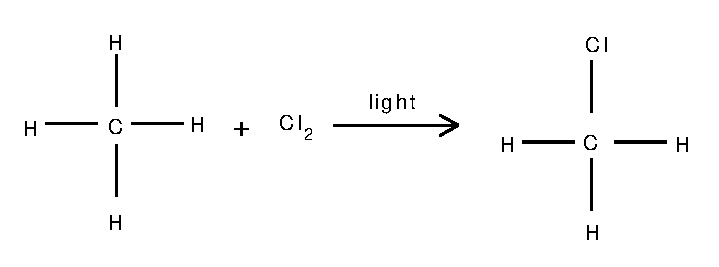
\includegraphics{../../epsimages/substitution_rxn.eps}
 % substitution_rxn.eps: 0x0 pixel, 300dpi, 0.00x0.00 cm, bb=3 6 332 118
\end{center}


% \begin{center}
% \begin{pspicture}(-2,-1)(10,1)
% \rput(-1,0){\textbf{H}}
% \psline(-0.7,0)(-0.3,0)
% \rput(0,0){\textbf{C}}
% \psline(0,0.3)(0,0.7)
% \rput(0,1){\textbf{H}}
% \psline(0.3,0.05)(0.7,0.05)
% \psline(0.3,-0.05)(0.7,-0.05)
% \rput(1,0){\textbf{C}}
% \psline(1,0.3)(1,0.7)
% \rput(1,1){\textbf{H}}
% \psline(1.3,0)(1.7,0)
% \rput(2,0){\textbf{H}}
% \rput(3,0){\textbf{+}}
% \rput(4,0){\textbf{HBr}}
% \psline[arrows=->](4.7,0)(5.5,0)
% \rput(7,0){
% \rput(-1,0){\textbf{H}}
% \psline(-0.7,0)(-0.3,0)
% \rput(0,0){\textbf{C}}
% \psline(0,0.3)(0,0.7)
% \rput(0,1){\textbf{H}}
% \psline(0.3,0)(0.7,0)
% \rput(1,0){\textbf{C}}
% \psline(1,0.3)(1,0.7)
% \rput(1,1){\textbf{H}}
% \psline(1.3,0)(1.7,0)
% \rput(2,0){\textbf{Br}}
% \rput(0,-1){\textbf{H}}
% \rput(1,-1){\textbf{H}}
% \psline(0,-0.3)(0,-0.7)
% \psline(1,-0.3)(1,-0.7)
% }
% \end{pspicture}
% \end{center}
\caption{A substitution reaction}
\label{fig:organic:substitution}
\end{figure}
}

Halo-alkanes (also sometimes called \textit{alkyl halides}) that contain methane and chlorine are substances that can be used as anaesthetics during operations. One example is trichloromethane, also known as 'chloroform' (figure \ref{fig:om:chloroform}).

\begin{figure}[h]
\begin{center}
\begin{pspicture}(-1.5,-1.5)(3,1.5)
%\psgrid[gridcolor=lightgray]
\rput(0,0){\textbf{C}}
\rput(1,1){\textbf{Cl}}
\rput(-1,1){\textbf{H}}
\rput(-1,-1){\textbf{Cl}}
\rput(1,-1){\textbf{Cl}}
\psline(0.2,0.2)(0.8,0.8)
\psline(-0.2,0.2)(-0.8,0.8)
\psline(0.2,-0.2)(0.8,-0.8)
\psline(-0.2,-0.2)(-0.8,-0.8)
\rput(2.5,0){\textbf{CHCl$_{3}$}}
\end{pspicture}

\end{center}
\caption{Trichloromethane}
\label{fig:om:chloroform}
\end{figure}


\item{\textbf{Elimination reactions}

Saturated compounds can also undergo elimination reactions to become unsaturated (figure \ref{fig:organic:elimination}). In the example below, an atom of hydrogen and chlorine are eliminated from the original compound to form an unsaturated halo-alkene.\\

e.g. \rm${ClH_{2}C-CH_{2}Cl \rightarrow H_{2}C=CHCl + HCl}$

\begin{figure}[h]
\begin{center}
\begin{pspicture}(-3,-1)(10,2)
\rput(-1,0){\textbf{H}}
\psline(-0.7,0)(-0.3,0)
\rput(0,0){\textbf{C}}
\psline(0,0.3)(0,0.7)
\rput(0,1){\textbf{H}}
\psline(0.3,0)(0.7,0)
\rput(1,0){\textbf{C}}
\psline(1,0.3)(1,0.7)
\rput(1,1){\textbf{H}}
\psline(1.3,0)(1.7,0)
\rput(2,0){\textbf{}}
\rput(0,-1){\textbf{Cl}}
\rput(1,-1){\textbf{Cl}}
\psline(0,-0.3)(0,-0.7)
\psline(1,-0.3)(1,-0.7)
\rput(2,0){\textbf{H}}
\psline[arrows=->](2.7,0)(3.5,0)
\rput(5,0){
\rput(-1,0){\textbf{H}}
\psline(-0.7,0)(-0.3,0)
\rput(0,0){\textbf{C}}
\psline(0,0.3)(0,0.7)
\rput(0,1){\textbf{H}}
\psline(0.3,0.05)(0.7,0.05)
\psline(0.3,-0.05)(0.7,-0.05)
\rput(1,0){\textbf{C}}
\psline(1,0.3)(1,0.7)
\rput(1,1){\textbf{H}}
\psline(1.3,0)(1.7,0)
\rput(2,0){\textbf{Cl}}
\rput(3,0){\textbf{+}}
\rput(4,0){\textbf{HCl}}
}
\end{pspicture}
\end{center}
\caption{An elimination reaction}
\label{fig:organic:elimination}
\end{figure}
}
\item{\textbf{Oxidation reactions}
 
When alkanes are burnt in air, they react with the oxygen in air and heat is produced. This is called an oxidation or combustion reaction. Carbon dioxide and water are given off as products. Heat is also released during the reaction. The burning of alkanes provides most of the energy that is used by man.\\

e.g. \rm${CH_{4} + 2O_{2} \rightarrow CO_{2} + 2H_{2}O + heat}$
}

\end{enumerate}


\Exercise{The Alkanes}{

\begin{enumerate}
\item{Give the IUPAC name for each of the following alkanes:}
	\begin{enumerate}
	\item{CH$_{3}$CH$_{2}$CH$_{2}$CH$_{2}$CH$_{2}$CH$_{3}$}
	\item{
	\begin{pspicture}(-3,-1.5)(2,3.5)
	%\psgrid[gridcolor=lightgray]
	\rput(-2,0){\textbf{C}}
	\rput(-2,1){\textbf{H}}
	\rput(-2,-1){\textbf{H}}
	\rput(-3,0){\textbf{H}}


	\psline(-2.8,0)(-2.2,0)
	\psline(-2,0.2)(-2,0.8)
	\psline(-2,-0.2)(-2,-0.8)
	\psline(-1.8,0)(-1.2,0)
	\rput(-1,0){\textbf{C}}
	\psline(-0.8,0)(-0.2,0)
	\rput(0,0){\textbf{C}}
	\psline(0.2,0)(0.8,0)
	\rput(1,0){\textbf{C}}
	\psline(1.2,0)(1.8,0)
	\psline(-1,0.2)(-1,1.8)
	\rput(-1,2){\textbf{C}}
	\rput(-1,3){\textbf{H}}
	\psline(-1.2,2)(-1.8,2)
	\psline(-0.2,2)(-0.8,2)
	\psline(-1,2.2)(-1,2.8)
	\rput(-2,2){\textbf{H}}
	\rput(0,2){\textbf{H}}
	\psline(-1,-0.2)(-1,-0.8)
	\rput(-1,-1){\textbf{H}}
	\rput(0,1){\textbf{H}}
	\rput(0,-1){\textbf{H}}
	\psline(0,0.2)(0,0.8)
	\psline(0,-0.2)(0,-0.8)
	\psline(1,0.2)(1,0.8)
	\rput(1,1){\textbf{H}}
	\psline(1,-0.2)(1,-0.8)
	\rput(1,-1){\textbf{H}}
	\rput(2,0){\textbf{H}}
	\end{pspicture}
	}
\item{CH$_{3}$CH$_{3}$}
\end{enumerate}

\item{Give the structural formula for each of the following compounds:}
	\begin{enumerate}
	\item{octane}
	\item{3-methyl-hexane}
	\end{enumerate}


\item{Methane is one of the simplest alkanes and yet it is an important fuel source. Methane occurs naturally in wetlands, natural gas and permafrost. However, methane can also be produced when organic wastes (e.g. animal manure and decaying material) are broken down by bacteria under conditions that are anaerobic (there is no oxygen). The simplified reaction is shown below:

\begin{center}
Organic matter \rm${\rightarrow}$ Simple organic acids \rm${\rightarrow}$ Biogas
\end{center}

The organic matter could be carbohydrates, proteins or fats which are broken down by acid-forming bacteria into simple organic acids such as acetic acid or formic acid. Methane-forming bacteria then convert these acids into biogases such as methane and ammonia.\\

The production of methane in this way is very important because methane can be used as a fuel source. One of the advantages of methane over other fuels like coal, is that it produces more energy but with lower carbon dioxide emissions. The problem however, is that methane itself is a greenhouse gas and has a much higher global warming potential than carbon dioxide. So, producing methane may in fact have an even more dangerous impact on the environment.

\begin{enumerate}
\item{What is the structural formula of methane?}
\item{Write an equation to show the reaction that takes place when methane is burned as a fuel.}
\item{Explain what is meant by the statement that methane 'has a greater global warming potential than carbon dioxide'.}
\end{enumerate}
}

\item{Chlorine and ethane react to form chloroethane and hydrogen chloride.}
	\begin{enumerate}
	\item{Write a balanced chemical equation for this reaction, using molecular formulae.}
	\item{Give the structural formula of chloroethane.}
	\item{What type of reaction has taken place in this example?}
	\end{enumerate}

\item{Petrol (C$_{8}$H$_{18}$) is in fact not pure C$_{8}$H$_{18}$ but a mixture of various \textit{alkanes}. The 'octane rating' of petrol refers to the percentage of the petrol which is C$_{8}$H$_{18}$. For example, 93 octane fuel contains 93\% C$_{8}$H$_{18}$ and 7\% other alkanes. The \textit{isomer} of C$_{8}$H$_{18}$ referred to in the 'octane rating' is in fact not octane but 2,2,4-trimethylpentane.}
	\begin{enumerate}
	\item{Write an unbalanced equation for the chemical reaction which takes place when petrol (C$_{8}$H$_{18}$) burns in excess oxygen.}
	\item{Write the general formula of the \textit{alkanes}.}
	\item{Define the term \textit{structural isomer}.}
	\item{Use the information given in this question and your knowledge of naming organic compounds to deduce and draw the full structural formula for 2,2,4-trimethylpentane.}
(IEB pg 25) 
	\end{enumerate}
\end{enumerate}

}

\subsection{The alkenes}

In the alkenes, there is at least one double bond between two carbon atoms. This means that they are \textbf{unsaturated} and are \textit{more reactive} than the alkanes. The simplest alkene is ethene (also known as ethylene), which is shown in figure \ref{fig:om:ethene3rep}.

\begin{figure}[h]
\begin{center}

\begin{pspicture}(-3,-1)(8,2)
%\psgrid[gridcolor=lightgray]
\rput(-3,0){(a)}
\rput(-1,0){\textbf{C}}
\rput(0,0){\textbf{C}}
\psline(-0.8,-0.05)(-0.2,-0.05)
\psline(-0.8,0.05)(-0.2,0.05)
\psline(0.2,0.2)(0.7,0.7)
\psline(0.2,-0.2)(0.7,-0.7)
\psline(-1.2,0.2)(-1.7,0.7)
\psline(-1.2,-0.2)(-1.7,-0.7)
\rput(1,1){\textbf{H}}
\rput(1,-1){\textbf{H}}
\rput(-2,1){\textbf{H}}
\rput(-2,-1){\textbf{H}}
\rput(2,0){(b)}
\rput(3.5,0){\textbf{CH$_{2}$CH$_{2}$}}
\rput(5,0){(c)}
\rput(6,0){\textbf{C$_{2}$H$_{4}$}}
\end{pspicture}
\end{center}
\caption{The (a) structural, (b) condensed structural and (c) molecular structure representations of ethene}
\label{fig:om:ethene3rep}
\end{figure}

As with the alkanes, the alkenes also form a homologous series. They have the general formula C$_{n}$H$_{2n}$. The second alkene in the series would therefore be C$_{3}$H$_{6}$. This molecule is known as propene (figure \ref{fig:om:propene3rep}). Note that if an alkene has two double bonds, it is called a \textbf{diene} and if it has three double bonds it is called a \textbf{triene}.

\begin{figure}[h]
\begin{center}
\begin{pspicture}(-3,-1)(8,2)
%\psgrid[gridcolor=lightgray]
\rput(-3,0){(a)}
\rput(-2,0){\textbf{H}}
\rput(-1,0){\textbf{C}}
\rput(0,0){\textbf{C}}
\rput(1,0){\textbf{C}}
\rput(-1,1){\textbf{H}}
\rput(-1,-1){\textbf{H}}
\rput(0,1){\textbf{H}}
\rput(2,1){\textbf{H}}
\rput(2,-1){\textbf{H}}
\psline(-1.8,0)(-1.2,0)
\psline(-0.8,0)(-0.2,0)
\psline(0.2,0.05)(0.8,0.05)
\psline(0.2,-0.05)(0.8,-0.05)
\psline(-1,0.2)(-1,0.8)
\psline(-1,-0.2)(-1,-0.8)
\psline(0,0.2)(0,0.8)
\psline(1.2,0.2)(1.8,0.8)
\psline(1.2,-0.2)(1.8,-.8)
\rput(4,0){\textbf{CH$_{3}$CHCH$_{2}$}}
\rput(2.5,0){(b)}
\rput(7,0){\textbf{C$_{3}$H$_{6}$}}
\rput(6,0){(c)}
\end{pspicture}
\end{center}
\caption{The (a) structural, (b) condensed structural and (c) molecular structure representations of propene}
\label{fig:om:propene3rep}
\end{figure}

The alkenes have a variety of uses. Ethylene for example is a hormone in plants that stimulates the ripening of fruits and the opening of flowers. Propene is an important compound in the petrochemicals industry. It is used as a monomer to make polypropylene and is also used as a fuel gas for other industrial processes. 

\subsection{Naming the alkenes}

Similar rules will apply in naming the alkenes, as for the alkanes. 

Khan Academy video on naming alkenes: SIYAVULA-VIDEO:http://cnx.org/content/m39453/latest/#alkenes
\begin{wex}{Naming the alkenes}{Give the IUPAC name for the following compound:

\begin{center}
\begin{pspicture}(-3,-2)(2,2)
%\psgrid[gridcolor=lightgray]
\rput(-3,0){\textbf{H}}
\psline(-2.7,0)(-2.3,0)
\rput(-2,0){\textbf{C$_{(1)}$}}
\rput(-2,1){\textbf{H}}
\rput(-2,-1){\textbf{H}}
\psline(-2,0.3)(-2,0.7)
\psline(-2,-0.3)(-2,-0.7)
\psline(-1.7,0)(-1.3,0)
\rput(-1,0){\textbf{C$_{(2)}$}}
\psline(-1,0.3)(-1,0.7)
\rput(-1,1){\textbf{H}}
\psline(-0.7,0.05)(-0.3,0.05)
\psline(-0.7,-0.05)(-0.3, -0.05)
\rput(0,0){\textbf{C$_{(3)}$}}
\rput(0,1){\textbf{H}}
\psline(0,0.3)(0,0.7)
\psline(0.3,0)(0.7,0)
\rput(1,0){\textbf{C$_{(4)}$}}
\rput(1,1){\textbf{H}}
\rput(1,-1){\textbf{H}}
\psline(1,0.3)(1,0.7)
\psline(1,-0.3)(1,-0.7)
\rput(2,0){\textbf{H}}
\psline(1.3,0)(1.7,0)
\end{pspicture}
\end{center}
}

{\westep{Identify the functional group}
The compound is an alkene and will have the suffix -ene.
\westep{Find the longest carbon chain}
There are four carbon atoms in the longest chain and so the prefix for this compound will be 'but'.
\westep{Number the carbon atoms}
Remember that when there is a double or triple bond, the carbon atoms must be numbered so that the double or triple bond is at the lowest numbered carbon. In this case, it doesn't matter whether we number the carbons from the left to right, or from the right to left. The double bond will still fall between C$_{2}$ and C$_{3}$. The position of the bond will come just before the suffix in the compound's name.
\westep{Look for any branched groups, name them and give their position on the carbon chain}
There are no branched groups in this molecule.
\westep{Name the compound}
The name of this compound is \textbf{but-2-ene}.}
\end{wex}

\begin{wex}{Naming the alkenes}{Draw the structural formula for the organic compound 3-methyl-butene\\}
{\westep{Identify the functional group}
The suffix -ene means that this compound is an alkene and there must be a double bond in the molecule. There is no number immediately before the suffix which means that the double bond must be at the first carbon in the chain.
\westep{Determine the number of carbons in the longest chain}
The prefix for the compound is 'but' so there must be four carbons in the longest chain.
\westep{Look for any branched groups}
There is a methyl group at the third carbon atom in the chain.
\westep{Combine this information to draw the structural formula for this molecule.}

\begin{figure}[H]
\begin{center}
\begin{pspicture}(-3,-1)(2.5,3.2)
%\psgrid[gridcolor=lightgray]
\rput(-2,0){\textbf{C}}
\rput(-3,0.7){\textbf{H}}
\rput(-3,-0.7){\textbf{H}}
\psline(-2.2,0.2)(-2.8,0.5)
\psline(-2.2,-0.2)(-2.8,-0.5)
\psline(-1.8,0.05)(-1.2,0.05)
\psline(-1.8,-0.05)(-1.2,-0.05)
\rput(-1,0){\textbf{C}}
\rput(-1,1){\textbf{H}}
\psline(-1,0.2)(-1,0.8)
\psline(-0.2,0)(-0.8,0)
\rput(0,0){\textbf{C}}
\psline(0,-0.2)(0,-0.8)
\rput(0,-1){\textbf{H}}
\psline(0,0.2)(0,1.8)
\rput(0,2){\textbf{C}}
\psline(-0.2,2)(-0.8,2)
\rput(-1,2){\textbf{H}}
\psline(0,2.2)(0,2.8)
\rput(0,3){\textbf{H}}
\psline(0.2,2)(0.8,2)
\rput(1,2){\textbf{H}}
\psline(0.2,0)(0.8,0)
\rput(1,0){\textbf{C}}
\psline(1,0.2)(1,0.8)
\rput(1,1){\textbf{H}}
\psline(1,-0.2)(1,-0.8)
\rput(1,-1){\textbf{H}}
\psline(1.2,0)(1.8,0)
\rput(2,0){\textbf{H}}

\end{pspicture}
\end{center}
\end{figure}
}
\end{wex}

\begin{wex}{Naming the alkenes}{Give the IUPAC name for the following compound:
\begin{center}
\begin{pspicture}(-3,-1)(2,3)
%\psgrid[gridcolor=lightgray]
\rput(-3,0){\textbf{H}}
\psline(-2.7,0)(-2.3,0)
\rput(-2,0){\textbf{C$_{(1)}$}}
\rput(-2,1){\textbf{H}}
\psline(-2,0.3)(-2,0.7)
\psline(-1.7,0.05)(-1.3,0.05)
\psline(-1.7,-0.05)(-1.3,-0.05)
\rput(-1,0){\textbf{C$_{(2)}$}}
\psline(-1,0.3)(-1,0.7)
\rput(-1,1){\textbf{CH$_{2}$}}
\psline(-1,1.3)(-1,1.7)
\rput(-1,2){\textbf{CH$_{3}$}}
\psline(-0.7,0)(-0.3,0)
\rput(0,0){\textbf{C$_{(3)}$}}
\rput(0,1){\textbf{H}}
\psline(0,0.3)(0,0.7)
\psline(0.3,0.05)(0.7,0.05)
\psline(0.3,-0.05)(0.7,-0.05)
\rput(1,0){\textbf{C$_{(4)}$}}
\rput(1,1){\textbf{H}}
\psline(1,0.3)(1,0.7)
\rput(2,0){\textbf{H}}
\psline(1.3,0)(1.7,0)
\end{pspicture}
\end{center}
}

{\westep{Identify the functional group}
The compound is an alkene and will have the suffix -ene. There is a double bond between the first and second carbons and also between the third and forth carbons. The organic compound is therefore a 'diene'.
\westep{Find the longest carbon chain and number the carbon atoms}
There are four carbon atoms in the longest chain and so the prefix for this compound will be 'but'. The carbon atoms are numbered 1 to 4 in the diagram above. Remember that the main carbon chain must contain both the double bonds.
\westep{Look for any branched groups, name them and give their position on the carbon chain}
There is an ethyl group on the second carbon.
\westep{Name the compound}
The name of this compound is \textbf{2-ethyl-but-1,3-diene}.}
\end{wex}



\Exercise{Naming the alkenes\\}{
Give the IUPAC name for each of the following alkenes:

\begin{enumerate}
\item{CH$_{2}$CHCH$_{2}$CH$_{2}$CH$_{3}$}
\item{CH$_{3}$CHCHCH$_{3}$}
\item{}

\begin{pspicture}(0,-1.3)(4,1.3)
\rput(0,0){H}
\psline(0.3,0)(0.7,0)

\rput(1,0){C}
\psline(1,0.3)(1,0.7)
\rput(1,1){H}
\psline(1.3,0.05)(1.7,0.05)
\psline(1.3,-0.05)(1.7,-0.05)
\rput(1,0){
\rput(1,0){C}
\psline(1.3,0.05)(1.7,0.05)
\psline(1.3,-0.05)(1.7,-0.05)
}
\rput(2,0){
\rput(1,0){C}
\psline(1,0.3)(1,0.7)
\rput(1,1){H}
\psline(1.3,0)(1.7,0)
}
\rput(3,0){
\rput(1,0){C}
\psline(1,0.3)(1,0.7)
\rput(1,1){H}
\psline(1,-0.3)(1,-0.7)
\rput(1,-1){H}
\psline(1.3,0)(1.7,0)
}
\rput(5,0){H}
\end{pspicture}

\end{enumerate}
}

\subsection{The properties of the alkenes}

The properties of the alkenes are very similar to those of the alkanes, except that the alkenes are more reactive because they are unsaturated. As with the alkanes, compounds that have four or less carbon atoms are gases at room temperature, while those with five or more carbon atoms are liquids.

\subsection{Reactions of the alkenes}

Alkenes can undergo \textbf{addition reactions} because they are unsaturated. They readily react with hydrogen, water and the halogens. The double bond is broken and a single, saturated bond is formed. A new group is then added to one or both of the carbon atoms that previously made up the double bond. The following are some examples:

\begin{enumerate}
\item{\textbf{Hydrogenation reactions} 

A catalyst such as platinum is normally needed for these reactions

\rm${H_{2}C=CH_{2} + H_{2} \rightarrow H_{3}C-CH_{3}}$ (figure \ref{fig:organic:hydrogenation})

\begin{figure}[h]
\begin{center}
\begin{pspicture}(-2,-0.5)(10,1.5)
\rput(-1,0){\textbf{H}}
\psline(-0.7,0)(-0.3,0)
\rput(0,0){\textbf{C}}
\psline(0,0.3)(0,0.7)
\rput(0,1){\textbf{H}}
\psline(0.3,0.05)(0.7,0.05)
\psline(0.3,-0.05)(0.7,-0.05)
\rput(1,0){\textbf{C}}
\psline(1,0.3)(1,0.7)
\rput(1,1){\textbf{H}}
\psline(1.3,0)(1.7,0)
\rput(2,0){\textbf{H}}
\rput(3,0){\textbf{+}}
\rput(4,0){\textbf{H$_{2}$}}
\psline[arrows=->](4.7,0)(5.5,0)
\rput(7,0){
\rput(-1,0){\textbf{H}}
\psline(-0.7,0)(-0.3,0)
\rput(0,0){\textbf{C}}
\psline(0,0.3)(0,0.7)
\rput(0,1){\textbf{H}}
\psline(0.3,0)(0.7,0)
\rput(1,0){\textbf{C}}
\psline(1,0.3)(1,0.7)
\rput(1,1){\textbf{H}}
\psline(1.3,0)(1.7,0)
\rput(2,0){\textbf{H}}
\rput(0,-1){\textbf{H}}
\rput(1,-1){\textbf{H}}
\psline(0,-0.3)(0,-0.7)
\psline(1,-0.3)(1,-0.7)
}
\end{pspicture}
\end{center}
\caption{A hydrogenation reaction}
\label{fig:organic:hydrogenation}
\end{figure}
}

\item{\textbf{Halogenation reactions}

\rm${CH_{2}=CH_{2} + HBr \rightarrow CH_{3}-CH_{2}-Br}$ (figure \ref{fig:organic:halogenation})

\begin{figure}[h]
\begin{center}
\begin{pspicture}(-2,-1)(10,1.5)
\rput(-1,0){\textbf{H}}
\psline(-0.7,0)(-0.3,0)
\rput(0,0){\textbf{C}}
\psline(0,0.3)(0,0.7)
\rput(0,1){\textbf{H}}
\psline(0.3,0.05)(0.7,0.05)
\psline(0.3,-0.05)(0.7,-0.05)
\rput(1,0){\textbf{C}}
\psline(1,0.3)(1,0.7)
\rput(1,1){\textbf{H}}
\psline(1.3,0)(1.7,0)
\rput(2,0){\textbf{H}}
\rput(3,0){\textbf{+}}
\rput(4,0){\textbf{HBr}}
\psline[arrows=->](4.7,0)(5.5,0)
\rput(7,0){
\rput(-1,0){\textbf{H}}
\psline(-0.7,0)(-0.3,0)
\rput(0,0){\textbf{C}}
\psline(0,0.3)(0,0.7)
\rput(0,1){\textbf{H}}
\psline(0.3,0)(0.7,0)
\rput(1,0){\textbf{C}}
\psline(1,0.3)(1,0.7)
\rput(1,1){\textbf{H}}
\psline(1.3,0)(1.7,0)
\rput(2,0){\textbf{Br}}
\rput(0,-1){\textbf{H}}
\rput(1,-1){\textbf{H}}
\psline(0,-0.3)(0,-0.7)
\psline(1,-0.3)(1,-0.7)
}
\end{pspicture}
\end{center}
\caption{A halogenation reaction}
\label{fig:organic:halogenation}
\end{figure}
}

\item{\textbf{The formation of alcohols}

\rm${CH_{2}=CH_{2} + H_{2}O \rightarrow CH_{3}-CH_{2}-OH}$ (figure \ref{fig:organic:forming alcohols})

\begin{figure}[h]
\begin{center}
\begin{pspicture}(-2,-1)(10,1.5)
\rput(-1,0){\textbf{H}}
\psline(-0.7,0)(-0.3,0)
\rput(0,0){\textbf{C}}
\psline(0,0.3)(0,0.7)
\rput(0,1){\textbf{H}}
\psline(0.3,0.05)(0.7,0.05)
\psline(0.3,-0.05)(0.7,-0.05)
\rput(1,0){\textbf{C}}
\psline(1,0.3)(1,0.7)
\rput(1,1){\textbf{H}}
\psline(1.3,0)(1.7,0)
\rput(2,0){\textbf{H}}
\rput(3,0){\textbf{+}}
\rput(4,0){\textbf{H$_{2}$O}}
\psline[arrows=->](4.7,0)(5.5,0)
\rput(7,0){
\rput(-1,0){\textbf{H}}
\psline(-0.7,0)(-0.3,0)
\rput(0,0){\textbf{C}}
\psline(0,0.3)(0,0.7)
\rput(0,1){\textbf{H}}
\psline(0.3,0)(0.7,0)
\rput(1,0){\textbf{C}}
\psline(1,0.3)(1,0.7)
\rput(1,1){\textbf{H}}
\psline(1.3,0)(1.7,0)
\rput(2,0){\textbf{OH}}
\rput(0,-1){\textbf{H}}
\rput(1,-1){\textbf{H}}
\psline(0,-0.3)(0,-0.7)
\psline(1,-0.3)(1,-0.7)
}
\end{pspicture}
\end{center}
\caption{The formation of an alcohol}
\label{fig:organic:forming alcohols}
\end{figure}
}
\end{enumerate}

\Exercise{The Alkenes\\}{
\begin{enumerate}
\item{Give the IUPAC name for each of the following organic compounds:}
	\begin{enumerate}
	\item{
\begin{pspicture}(-3,-3)(2,2)
	%\psgrid[gridcolor=lightgray]
	\rput(-2,0){\textbf{C}}
	\rput(-2,1){\textbf{H}}
	\rput(-2,-1){\textbf{H}}
	\rput(-3,0){\textbf{H}}
	\psline(-2.8,0)(-2.2,0)
	\psline(-2,0.2)(-2,0.8)
	\psline(-2,-0.2)(-2,-0.8)
	\psline(-1.8,0)(-1.2,0)
	\rput(-1,0){\textbf{C}}
	\psline(-0.8,0.05)(-0.2,0.05)
	\psline(-0.8,-0.05)(-0.2,-0.05)
	\rput(0,0){\textbf{C}}
	\psline(0.2,0)(0.8,0)
	\rput(1,0){\textbf{C}}
	\psline(1.2,0)(1.8,0)
	\psline(-1,-0.2)(-1,-0.8)
	\rput(-1,-1){\textbf{H}}
	\rput(0,-1){\textbf{H}}
	\psline(0,-0.2)(0,-0.8)
	\psline(1,0.2)(1,0.8)
	\rput(1,1){\textbf{H}}
	\psline(1,-0.2)(1,-1.8)
	\rput(1,-2){\textbf{C}}
	\rput(1,-3){\textbf{H}}
	\rput(0,-2){\textbf{H}}
	\rput(2,-2){\textbf{H}}
	\psline(0.8,-2)(0.2,-2)
	\psline(1.8,-2)(1.2,-2)
	\psline(1,-2.2)(1,-2.8)
	\rput(2,0){\textbf{H}}
	\end{pspicture}
	}
	\item{CH$_{3}$CHCH$_{2}$}
	\end{enumerate}

\item{Refer to the data table below which shows the melting point and boiling point for a number of different organic compounds.

\begin{center}
\begin{tabular}{|l|l|c|c|}\hline
\textbf{Formula} & \textbf{Name} & \textbf{Melting point ($^{0}$C)} & \textbf{Boiling point ($^{0}$C)}\\\hline
C$_{4}$H$_{10}$ & Butane & -138 & -0.5 \\\hline
C$_{5}$H$_{12}$ & Pentane & -130 & 36 \\\hline
C$_{6}$H$_{14}$ & Hexane & -95 & 69 \\\hline
C$_{4}$H$_{8}$ & Butene & -185 & -6 \\\hline
C$_{5}$H$_{10}$ & Pentene & -138 & 30 \\\hline
C$_{6}$H$_{12}$ & Hexene & -140 & 63 \\\hline
\end{tabular}
\end{center}
	\begin{enumerate}
	\item{At room temperature (approx. 25$^{0}$C), which of the organic compounds in the table are:
		\begin{enumerate}
		\item{gases}
		\item{liquids}
		\end{enumerate}
}
	\item{In the alkanes...
		\begin{enumerate}
		\item{Describe what happens to the melting point and boiling point as the number of carbon atoms in the compound increases.}
		\item{Explain why this is the case.}
		\end{enumerate}
}
	\item{If you look at an alkane and an alkene that have the same number of carbon atoms...
		\begin{enumerate}
		\item{How do their melting points and boiling points compare?}
		\item{Can you explain why their melting points and boiling points are different?}
		\end{enumerate}
}
	\item{Which of the compounds, hexane or hexene, is more reactive? Explain your answer.}
	\end{enumerate}
}

\item{
The following reaction takes place:\\
\begin{center}
\rm${CH_{3}CHCH_{2} + H_{2} \rightarrow CH_{3}CH_{2}CH_{3}}$
\end{center}

\begin{enumerate}
\item{Give the name of the organic compound in the reactants.}
\item{What is the name of the product?}
\item{What type of reaction is this?}
\item{Which compound in the reaction is a saturated hydrocarbon?}
\end{enumerate}

}
\end{enumerate}
}


\subsection{The Alkynes}

In the alkynes, there is at least one triple bond between two of the carbon atoms. They are unsaturated compounds and are therefore highly reactive. Their general formula is C$_{n}$H$_{2n-2}$. The simplest alkyne is ethyne (figure \ref{fig:om:ethyne}), also known as acetylene. Many of the alkynes are used to synthesise other chemical products.

\begin{figure}[h]
\begin{center}


\begin{pspicture}(-2,-0.5)(1,0.5)
%\psgrid[gridcolor=lightgray]
\rput(-2,0){\textbf{H}}
\rput(-1,0){\textbf{C}}
\rput(0,0){\textbf{C}}
\rput(1,0){\textbf{H}}
\psline(-1.8,0)(-1.2,0)
\psline(-0.8,0.075)(-0.2,0.075)
\psline(-0.8,0)(-0.2,0)
\psline(-0.8,-0.075)(-0.2,-0.075)
\psline(0.2,0)(0.8,0)
\end{pspicture}
\end{center}
\caption{Ethyne (acetylene)}
\label{fig:om:ethyne}
\end{figure}

\begin{IFact}{
The raw materials that are needed to make acetylene are calcium carbonate and coal. Acetylene can be produced through the following reactions:
\begin{center}
\rm${CaCO_{3} \rightarrow CaO}$

\rm${CaO + 3C \rightarrow CaC_{2} + CO}$

\rm${CaC_{2} + 2H_{2}O \rightarrow Ca(OH)_{2} + C_{2}H_{2}}$
\end{center}

An important use of acetylene is in oxyacetylene gas welding. The fuel gas burns with oxygen in a torch. An incredibly high heat is produced, and this is enough to melt metal.
}
\end{IFact}

\subsection{Naming the alkynes}

The same rules will apply as for the alkanes and alkenes, except that the suffix of the name will now be -yne.

\begin{wex}{Naming the alkynes}{Give the IUPAC name for the following compound:

\begin{figure}[H]
\begin{center}
\begin{pspicture}(-4,-1.5)(4,1)
%\psgrid[gridcolor=lightgray]
\rput(-3,0){\textbf{CH$_{3}$}}
\rput(-2,0){\textbf{CH}}
\psline(-2.6,0)(-2.4,0)
\rput(-1,0){\textbf{CH$_{2}$}}
\psline(-1.6,0)(-1.4,0)
\rput(-2,-1){\textbf{CH$_{3}$}}
\psline(-2,-0.3)(-2,-0.7)
\rput(0,0){\textbf{C}}
\psline(0.4,0)(0.6,0)
\rput(1,0){\textbf{C}}
\rput(2,0){\textbf{CH$_{3}$}}
\psline(0.4,0.075)(0.6,0.075)
\psline(0.4,0)(0.6,0)
\psline(0.4,-0.075)(0.6,-0.075)
\psline(1.4,0)(1.6,0)
\psline(-0.6,0)(-0.4,0)
\end{pspicture}
\end{center}
\end{figure}
}
{\westep{Identify the functional group}
There is a triple bond between two of the carbon atoms, so this compound is an alkyne. The suffix will be -yne. The triple bond is at the second carbon, so the suffix will in fact be 2-yne.\\
\westep{Find the longest carbon chain and give the compound the correct prefix}
If we count the carbons in a straight line, there are six. The prefix of the compound's name will be 'hex'.
\westep{Number the carbons in the longest chain}
In this example, you will need to number the carbons from right to left so that the triple bond is between carbon atoms with the lowest numbers.
\westep{Look for any branched groups, name them and show the number of the carbon atom to which the group is attached}
There is a methyl (CH$_{3}$) group attached to the fifth carbon (remember we have numbered the carbon atoms from right to left).
\westep{Combine the elements of the name into a single word in the following order: branched groups; prefix; name ending according to the functional group and its position along the longest carbon chain.}
If we follow this order, the name of the compound is \textbf{5-methyl-hex-2-yne}.
}
\end{wex}

\Exercise{The alkynes\\}{

Give the IUPAC name for each of the following organic compounds.

\begin{enumerate}
\item{
\begin{pspicture}(-3,-1.5)(3,1.5)
\rput(-3,0){\textbf{H}}
\psline(-2.7,0)(-2.3,0)
\rput(-2,0){\textbf{C}}
\psline(-2,0.3)(-2,0.7)
\rput(-2,1){\textbf{H}}
\psline(-2,-0.3)(-2,-0.7)
\rput(-2,-1){\textbf{H}}
\psline(-1.7,0)(-1.3,0)
\rput(-1,0){\textbf{C}}
\psline(-1,0.3)(-1,0.7)
\rput(-1,1){\textbf{CH$_{3}$}}
\psline(-1,-0.3)(-1,-0.7)
\rput(-1,-1){\textbf{H}}
\psline(-0.7,0)(-0.3,0)
\rput(0,0){\textbf{C}}
\psline(0.3,0.05)(0.7,0.05)
\psline(0.3,0)(0.7,0)
\psline(0.3,-0.05)(0.7,-0.05)
\rput(1,0){\textbf{C}}
\psline(1.3,0)(1.7,0)
\rput(2,0){\textbf{H}}
\end{pspicture}
}

\item{
C$_{2}$H$_{2}$
}

\item{
CH$_{3}$CH$_{2}$CCH
}
\end{enumerate}
}



% CHILD SECTION END 



% CHILD SECTION START 

\section{The Alcohols}

An alcohol is any organic compound where there is a \textit{hydroxyl} functional group (-OH) bound to a carbon atom. The general formula for a simple alcohol is C$_{n}$H$_{2n+1}$OH.\\

The simplest and most commonly used alcohols are methanol and ethanol (figure \ref{fig:om:metheth}).
\begin{figure}[h]
\begin{center}
\begin{pspicture}(-4,-1.5)(4,1.5)
%\psgrid[gridcolor=lightgray]
\rput(-2,0){\textbf{C}}
\rput(-3,0){\textbf{H}}
\rput(-1,0){\textbf{H}}
\rput(-2,1){\textbf{OH}}
\rput(-2,-1){\textbf{H}}
\psline(-2.8,0)(-2.2,0)
\psline(-1.8,0)(-1.2,0)
\psline(-2,0.2)(-2,0.8)
\psline(-2,-0.2)(-2,-0.8)
\rput(-3.5,1){\textbf{(a)}}

\rput(0,0){\textbf{H}}
\rput(1,0){\textbf{C}}
\rput(2,0){\textbf{C}}
\rput(3,0){\textbf{H}}
\rput(1,1){\textbf{H}}
\rput(1,-1){\textbf{H}}
\rput(2,1){\textbf{OH}}
\rput(2,-1){\textbf{H}}
\rput(3,0){\textbf{H}}
\psline(0.2,0)(0.8,0)
\psline(1.2,0)(1.8,0)
\psline(2.2,0)(2.8,0)
\psline(1,0.2)(1,0.8)
\psline(1,-0.2)(1,-0.8)
\psline(2,0.2)(2,0.8)
\psline(2,-0.2)(2,-0.8)
\rput(0,1){\textbf{(b)}}
\end{pspicture}
\end{center}
\caption{(a) methanol and (b) ethanol}
\label{fig:om:metheth}
\end{figure}

The alcohols have a number of different uses:

\begin{itemize}
\item{methylated spirits (surgical spirits) is a form of ethanol where methanol has been added}
\item{ethanol is used in alcoholic drinks}
\item{ethanol is used as an industrial solvent}
\item{methanol and ethanol can both be used as a fuel and they burn more cleanly than gasoline or diesel (refer to Grade 11 for more information on biofuels as an alternative energy resource.)}
\item{ethanol is used as a solvent in medical drugs, perfumes and vegetable essences}
\item{ethanol is an antiseptic}
\end{itemize}

\begin{IFact}

'Fermentation' refers to the conversion of sugar to alcohol using yeast (a fungus). The process of fermentation produces items such as wine, beer and yoghurt. To make wine, grape juice is fermented to produce alcohol. This reaction is shown below:
\begin{center}
\rm${C_{6}H_{12}O_{6} \rightarrow 2CO_{2} + 2C_{2}H_{5}OH + energy}$
\end{center}
\end{IFact}

\begin{IFact}{
Ethanol is a diuretic. In humans, ethanol reduces the secretion of a hormone called antidiuretic hormone (ADH). The role of ADH is to control the amount of water that the body retains. When this hormone is not secreted in the right quantities, it can cause dehyration because too much water is lost from the body in the urine. This is why people who drink too much alcohol can become dehydrated, and experience symptoms such as headaches, dry mouth, and lethargy. Part of the reason for the headaches is that dehydration causes the brain to shrink away from the skull slightly. The effects of drinking too much alcohol can be reduced by drinking lots of water.}
\end{IFact}

\subsection{Naming the alcohols}
\label{subsec:om:alcoholnaming}

The rules used to name the alcohols are similar to those already discussed for the other compounds, except that the suffix of the name will be different because the compound is an alcohol.
Khan Academy video on alcohols: SIYAVULA-VIDEO:http://cnx.org/content/m39455/latest/#alcohols
\begin{wex}{Naming alcohols 1}{Give the IUPAC name for the following organic compound

\begin{figure}[H]
\begin{center}
\begin{pspicture}(-3,-1.5)(3,1.5)
%\psgrid[gridcolor=lightgray]
\rput(-2,0){\textbf{H}}
\psline(-1.8,0)(-1.2,0)
\rput(-1,0){\textbf{C$_{1}$}}
\psline(-1,0.2)(-1,0.8)
\rput(-1,1){\textbf{H}}
\psline(-1,-0.2)(-1,-0.8)
\rput(-1,-1){\textbf{H}}
\psline(-0.2,0)(-0.8,0)
\rput(0,0){\textbf{C$_{2}$}}
\psline(0,0.2)(0,0.8)
\rput(0,1){\textbf{OH}}
\psline(0,-0.2)(0,-0.8)
\rput(0,-1){\textbf{H}}
\psline(0.2,0)(0.8,0)
\rput(1,0){\textbf{C$_{3}$}}
\psline(1,0.2)(1,0.8)
\rput(1,1){\textbf{H}}
\psline(1,-0.2)(1,-0.8)
\rput(1,-1){\textbf{H}}
\psline(1.2,0)(1.8,0)
\rput(2,0){\textbf{H}}
\end{pspicture}
\end{center}
\end{figure}
}
{\westep{Identify the functional group}
The compound has an -OH (hydroxyl) functional group and is therefore an alcohol. The compound will have the suffix -ol.\westep{Find the longest carbon chain}
There are three carbons in the longest chain. The prefix for this compound will be 'prop'. Since there are only single bonds between the carbon atoms, the suffix becomes 'propan' (similar to the alkane 'propane').
\westep{Number the carbons in the carbon chain}
In this case, it doesn't matter whether you start numbering from the left or right. The hydroxyl group will still be attached to the middle carbon atom, numbered '2'.
\westep{Look for any branched groups, name them and give their position on the carbon chain.}
There are no branched groups in this compound, but you still need to indicate the position of the hydroxyl group on the second carbon. The suffix will be -2-ol because the hydroxyl group is attached to the second carbon.
\westep{Combine the elements of the compound's name into a single word in the order of branched groups; prefix; name ending according to the functional group.}
The compound's name is propan-2-ol.
}
\end{wex}

\begin{wex}{Naming alcohols 2}{Give the IUPAC name for the following compound:

\begin{figure}[H]
\begin{center}
\begin{pspicture}(-3,-2)(3,2)
%\psgrid[gridcolor=lightgray]
\rput(-2,0){\textbf{H}}
\psline(-1.8,0)(-1.2,0)
\rput(-1,0){\textbf{C$_{1}$}}
\psline(-1,0.2)(-1,0.8)
\rput(-1,1){\textbf{OH}}
\psline(-1,-0.2)(-1,-0.8)
\rput(-1,-1){\textbf{H}}
\psline(-0.2,0)(-0.8,0)
\rput(0,0){\textbf{C$_{2}$}}
\psline(0,0.2)(0,0.8)
\rput(0,1){\textbf{OH}}
\psline(0,-0.2)(0,-0.8)
\rput(0,-1){\textbf{H}}
\psline(0.2,0)(0.8,0)
\rput(1,0){\textbf{C$_{3}$}}
\psline(1,0.2)(1,0.8)
\rput(1,1){\textbf{H}}
\psline(1,-0.2)(1,-0.8)
\rput(1,-1){\textbf{H}}
\psline(1.2,0)(1.8,0)
\rput(2,0){\textbf{C$_{4}$}}
\psline(2,0.2)(2,0.8)
\rput(2,1){\textbf{H}}
\psline(2,-0.2)(2,-0.8)
\rput(2,-1){\textbf{H}}
\psline(2.2,0)(2.8,0)
\rput(3,0){\textbf{H}}
\end{pspicture}
\end{center}
\end{figure}
}
{\westep{Identify the functional group}
The compound has an -OH (hydroxyl) functional group and is therefore an alcohol. There are \textit{two} hydroxyl groups in the compound, so the suffix will be -diol.
\westep{Find the longest carbon chain}
There are four carbons in the longest chain. The prefix for this compound will be 'butan'. 
\westep{Number the carbons in the carbon chain}
The carbons will be numbered from left to right so that the two hydroxyl groups are attached to carbon atoms with the lowest numbers.
\westep{Look for any branched groups, name them and give their position on the carbon chain.}
There are no branched groups in this compound, but you still need to indicate the position of the hydroxyl groups on the first and second carbon atoms. The suffix will therefore become 1,2-diol.
\westep{Combine the elements of the compound's name into a single word in the order of branched groups; prefix; name ending according to the functional group.}
The compound's name is butan-1,2-diol.
}
\end{wex}
 
\Exercise{Naming the alcohols\\}{
\begin{enumerate}
\item{Give the structural formula of each of the following organic compounds:}
	\begin{enumerate}
	\item{pentan-3-ol}
	\item{butan-2,3-diol}
	\item{2-methyl-propanol}
	\end{enumerate}
\item{Give the IUPAC name for each of the following:}
	\begin{enumerate}
	\item{CH$_{3}$CH$_{2}$CH(OH)CH$_{3}$}
	\item{
\begin{pspicture}(0,-1.3)(5,1.3)
\rput(0,0){CH$_{3}$}
\psline(0.3,0)(0.7,0)
\rput(1,0){C}
\psline(1,0.3)(1,0.7)
\rput(1,1){H}
\psline(1,-0.3)(1,-0.7)
\rput(1,-1){OH}
\psline(1.3,0)(1.7,0)
\rput(2,0){CH$_{2}$}
\psline(2.3,0)(2.7,0)
\rput(3,0){CH$_{2}$}
\psline(3.3,0)(3.7,0)
\rput(4,0){CH$_{3}$}
\end{pspicture}
}
	\end{enumerate}
\end{enumerate}
}

\subsection{Physical and chemical properties of the alcohols}
\label{sec:om:physchem}

The hydroxyl group affects the \textbf{solubility} of the alcohols. The hydroxyl group generally makes the alcohol molecule \textit{polar} and therefore more likely to be \textbf{soluble} in water. However, the carbon chain resists solubility, so there are two opposing trends in the alcohols. Alcohols with shorter carbon chains are usually more soluble than those with longer carbon chains.\\

Alcohols tend to have higher \textbf{boiling points} than the hydrocarbons because of the strong hydrogen bond between hydrogen and oxygen atoms. \\

Alcohols can show either \textbf{acidic} or \textbf{basic} properties because of the hydroxyl group. They also undergo oxidation reactions to form aldehydes, ketones and carboxylic acids.


\Activity{Case Study}{The uses of the alcohols}{Read the extract below and then answer the questions that follow:\\

The alcohols are a very important group of organic compounds, and they have a variety of uses. Our most common use of the word 'alcohol' is with reference to alcoholic drinks. The alcohol in drinks is in fact \textbf{ethanol}. But ethanol has many more uses apart from alcoholic drinks! When ethanol burns in air, it produces carbon dioxide, water and energy and can therefore be used as a fuel on its own, or in mixtures with petrol. Because ethanol can be produced through fermentation, this is a useful way for countries without an oil industry to reduce imports of petrol. Ethanol is also used as a solvent in many perfumes and cosmetics.\\

\textbf{Methanol} can also be used as a fuel, or as a petrol additive to improve combustion. Most methanol is used as an industrial feedstock, in other words it is used to make other things such as methanal (formaldehyde), ethanoic acid and methyl esters. In most cases, these are then turned into other products.\\

\textbf{Propan-2-ol} is another important alcohol, which is used in a variety of applications as a solvent.\\

\textbf{Questions}

\begin{enumerate}
\item{Give the structural formula for propan-2-ol.}
\item{Write a balanced chemical equation for the combustion reaction of ethanol.}
\item{Explain why the alcohols are good solvents.}
\end{enumerate}
}



% CHILD SECTION END 



% CHILD SECTION START 

\section{Carboxylic Acids}
\label{sec:om:carboxylic}

Carboxylic acids are organic acids that are characterised by having a carboxyl group, which has the formula -(C=O)-OH, or more commonly written as -COOH. In a carboxyl group, an oxygen atom is double-bonded to a carbon atom, which is also bonded to a hydroxyl group. The simplest carboxylic acid, methanoic acid, is shown in figure \ref{fig:om:methanoic acid}. The IUPAC suffix for carboxylic acids is -anoic acid.

\begin{figure}[h]
\begin{center}
\begin{pspicture}(-3,-1.5)(3,1.5)
%\psgrid[gridcolor=lightgray]
\rput(0,0){\textbf{C}}
\psline(-0.05,0.2)(-0.05,0.8)
\psline(0.05,0.2)(0.05,0.8)
\rput(0,1){\textbf{O}}
\psline(-0.2,-0.2)(-0.6,-0.6)
\rput(-0.8,-0.8){\textbf{H}}
\psline(0.2,-0.2)(0.6,-0.6)
\rput(0.8,-0.8){\textbf{OH}}
\end{pspicture}
\caption{Methanoic acid}
\label{fig:om:methanoic acid}
\end{center}
\end{figure}

Carboxylic acids are widespread in nature. Methanoic acid (also known as \textit{formic acid}) has the formula HCOOH and is found in insect stings. Ethanoic acid (CH$_{3}$COOH), or \textit{acetic acid}, is the main component of vinegar. More complex organic acids also have a variety of different functions. Benzoic acid (C$_{6}$H$_{5}$COOH) for example, is used as a food preservative.

\begin{IFact}

A certain type of ant, called formicine ants, manufacture and secrete formic acid, which is used to defend themselves against other organisms that might try to eat them.
\end{IFact}

\subsection{Physical Properties}
\label{sec:om:physicalproperties}

Carboxylic acids are \textbf{weak acids}, in other words they only dissociate partially. Why does the carboxyl group have acidic properties? In the carboxyl group, the hydrogen tends to separate itself from the oxygen atom. In other words, the carboxyl group becomes a source of positively-charged hydrogen ions (H$^{+}$). This is shown in figure \ref{fig:om:dissociation carboxylic acid}.

\begin{figure}[h]
\begin{center}
\begin{pspicture}(-6,-2)(7,1.5)
%\psgrid[gridcolor=lightgray]
\rput(-5,0){\textbf{H}}
\psline(-4.8,0)(-4.2,0)
\rput(-4,0){\textbf{C}}
\psline(-4,0.2)(-4,0.8)
\rput(-4,1){\textbf{H}}
\psline(-4,-0.2)(-4,-0.8)
\rput(-4,-1){\textbf{H}}
\psline(-3.2,0)(-3.8,0)
\rput(-3,0){\textbf{C}}
\psline(-2.8,0.2)(-2.2,0.6)
\psline(-2.9,0.3)(-2.3,0.7)
\rput(-2,0.8){\textbf{O}}
\psline(-2.8,-0.2)(-2.2,-0.6)
\rput(-1.8,-0.8){\textbf{OH}}
\psline[arrows=->](-1,0.05)(0,0.05)
\psline[arrows=->](0,-0.05)(-1,-0.05)
\rput(6,0){
\rput(-5,0){\textbf{H}}
\psline(-4.8,0)(-4.2,0)
\rput(-4,0){\textbf{C}}
\psline(-4,0.2)(-4,0.8)
\rput(-4,1){\textbf{H}}
\psline(-4,-0.2)(-4,-0.8)
\rput(-4,-1){\textbf{H}}
\psline(-3.2,0)(-3.8,0)
\rput(-3,0){\textbf{C}}
\psline(-2.8,0.2)(-2.2,0.6)

\psline(-2.9,0.3)(-2.3,0.7)
\rput(-2,0.8){\textbf{O}}
\psline(-2.8,-0.2)(-2.2,-0.6)
\rput(-1.8,-0.8){\textbf{O$^{-}$}}
}
\rput(4.7,0){\textbf{+}}
\rput(5.5,0){\textbf{H$^{+}$}}
\rput(-4,-1.5){\textbf{Acetic acid}}
\rput(2,-1.5){\textbf{Acetate ion}}
\rput(5.2,-1.5){\textbf{Hydrogen ion}}
\end{pspicture}
\end{center}
\caption{The dissociation of a carboxylic acid}
\label{fig:om:dissociation carboxylic acid}
\end{figure}


\Exercise{Carboxylic acids}{
\begin{enumerate}
\item{Refer to the table below which gives information about a number of carboxylic acids, and then answer the questions that follow.

\begin{center}
\begin{tabular}{|p{2.4cm}|p{1.2cm}|p{1.2cm}|p{1.2cm}|p{1.2cm}|p{1.2cm}|}\hline
\textbf{Formula} & \textbf{Common name} & \textbf{Source} & \textbf{IUPAC name} & \textbf{melting point} ($^{0}$C) & \textbf{boiling point} ($^{0}$C)\\\hline  
& formic acid & ants & methanoic acid & 8.4 & 101\\\hline
CH$_{3}$CO$_{2}$H & & vinegar & ethanoic acid & 16.6 & 118\\\hline
 & propionic acid & milk & propanoic acid & -20.8 & 141\\\hline
CH$_{3}$(CH$_{2}$)$_{2}$CO$_{2}$H & butyric acid & butter & & -5.5 & 164\\\hline
 & valeric acid & valerian root & pentanoic acid & -34.5 & 186\\\hline
CH$_{3}$(CH$_{2}$)$_{4}$CO$_{2}$H & caproic acid & goats & & -4 & 205\\\hline
 & enanthic acid & vines & & -7.5 & 223\\\hline
CH$_{3}$(CH$_{2}$)$_{6}$CO$_{2}$H & caprylic acid & goats & & 16.3 & 239\\\hline
\end{tabular}
\end{center}

	\begin{enumerate}
	\item{Fill in the missing spaces in the table by writing the formula, common name or IUPAC name.}
	\item{Draw the structural formula for butyric acid.}
	\item{Give the molecular formula for caprylic acid.}
	\item{Draw a graph to show the relationship between molecular mass (on the x-axis) and boiling point (on the y-axis)}
		\begin{enumerate}
		\item{Describe the trend you see.}
		\item{Suggest a reason for this trend.}
		\end{enumerate}
	\end{enumerate}
}

\end{enumerate}
}

\subsection{Derivatives of carboxylic acids: The esters}

When an alcohol reacts with a carboxylic acid, an \textbf{ester} is formed. Most esters have a characteristic and pleasant smell. In the reaction, the hydrogen atom from the hydroxyl group, and an OH from the carboxlic acid, form a molecule of water. A new bond is formed between what remains of the alcohol and acid. The name of the ester is a combination of the names of the alcohol and carboxylic acid. The suffix for an ester is -oate. An example is shown in figure \ref{fig:om:ester}.

\begin{figure}[h]
\begin{center}
\begin{pspicture}(-8,-2)(8,2)
%\psgrid[gridcolor=lightgray]
\rput(-8,0){\textbf{H}}
\psline(-7.8,0)(-7.2,0)
\rput(-7,0){\textbf{C}}
\psline(-7,0.2)(-7,0.8)
\rput(-7,1){\textbf{H}}
\psline(-7,-0.2)(-7,-0.8)
\rput(-7,-1){\textbf{H}}
\psline(-6.8,0)(-6.2,0)
\rput(-6,0){\textbf{O}}
\psline(-5.8,0)(-5.2,0)
\rput(-5,0){\textbf{H}}
\rput(-4.5,0){\textbf{+}}
\rput(-4,0){\textbf{H}}
\psline(-3.8,0)(-3.2,0)
\rput(-3,0){\textbf{O}}
\psline(-2.8,0)(-2.2,0)
\rput(-2,0){\textbf{C}}
\psline(-2.05,0.2)(-2.05,0.8)
\psline(-1.95,0.2)(-1.95,0.8)
\psline(-1.8,0)(-1.2,0)
\rput(-1,0){\textbf{H}}
\rput(-2,1){\textbf{O}}
\psline[arrows=->](-0.5,0)(0.5,0)
\rput(9,0){
\rput(-8,0){\textbf{H}}
\psline(-7.8,0)(-7.2,0)
\rput(-7,0){\textbf{C}}
\psline(-7,0.2)(-7,0.8)
\rput(-7,1){\textbf{H}}
\psline(-7,-0.2)(-7,-0.8)
\rput(-7,-1){\textbf{H}}
\psline(-6.8,0)(-6.2,0)
\rput(-6,0){\textbf{O}}
\psline(-5.8,0)(-5.2,0)
}
\rput(6,0){
\rput(-2,0){\textbf{C}}
\psline(-2.05,0.2)(-2.05,0.8)
\psline(-1.95,0.2)(-1.95,0.8)
\psline(-1.8,0)(-1.2,0)
\rput(-1,0){\textbf{H}}
\rput(-2,1){\textbf{O}}
}
\rput(5.5,0){\textbf{+}}
\rput(6.3,0){\textbf{H$_{2}$O}}
\rput(-6.5,-1.7){\textbf{methanol}}
\rput(-2.5,-1.7){\textbf{methanoic acid}}
\rput(2.5,-1.7){\textbf{methyl methanoate}}
\end{pspicture}
\end{center}
\caption{The formation of an ester and water from an alcohol and carboxylic acid}
\label{fig:om:ester}
\end{figure} 



% CHILD SECTION END 



% CHILD SECTION START 

\section{The Amino Group}

\label{sec:om:amino}

The amino group has the formula -NH$_{2}$ and consists of a nitrogen atom that is bonded to two hydrogen atoms, and to the carbon skeleton. Organic compounds that contain this functional group are called \textbf{amines}. One example is \textit{glycine}. Glycine belongs to a group of organic compounds called \textit{amino acids}, which are the building blocks of proteins.

\begin{figure}[h]
\begin{center}
\begin{pspicture}(-3,-1.5)(1.5,1.5)
%\psgrid[gridcolor=lightgray]
\rput(-2,0){\textbf{C}}
\psline(-2.2,0.2)(-2.6,0.6)
\psline(-2.25,0.15)(-2.65,0.55)
\rput(-2.8,0.8){\textbf{O}}
\psline(-2.2,-0.2)(-2.6,-0.6)
\rput(-2.8,-0.8){\textbf{HO}}
\psline(-1.8,0)(-1.2,0)
\rput(-1,0){\textbf{C}}
\psline(-1,0.2)(-1,0.8)
\rput(-1,1){\textbf{H}}
\psline(-1,-0.2)(-1,-0.8)
\rput(-1,-1){\textbf{H}}
\psline(-0.8,0)(-0.2,0)
\rput(0,0){\textbf{N}}
\psline(0.2,0.2)(0.6,0.6)
\rput(0.8,0.8){\textbf{H}}
\psline(0.2,-0.2)(0.6,-0.6)
\rput(0.8,-0.8){\textbf{H}}
\end{pspicture}
\end{center}
\caption{A molecule of glycine}
\label{fig:om:glycine}
\end{figure}


% CHILD SECTION END 



% CHILD SECTION START 

\section{The Carbonyl Group}
\label{sec:om:carbonyl}

The carbonyl group (-CO) consists of a carbon atom that is joined to an oxygen by a double bond. If the functional group is on the \textit{end} of the carbon chain, the organic compound is called a \textbf{ketone}. The simplest ketone is \textit{acetone}, which contains three carbon atoms. A ketone has the ending 'one' in its IUPAC name.

\Exercise{Carboxylic acids, esters, amines and ketones\\}{
\begin{enumerate}
\item{Look at the list of organic compounds in the table below:}
\begin{center}
\begin{tabular}{|l|l|}\hline
\textbf{Organic compound} & \textbf{Type of compound}\\\hline
CH$_{3}$CH$_{2}$CH$_{2}$COOH & \\\hline
NH$_{2}$CH$_{2}$COOH & \\\hline
propyl ethanoate & \\\hline
CH$_{3}$CHO & \\\hline
\end{tabular}
\end{center}

	\begin{enumerate}
	\item{Complete the table by identifying each compound as either a carboxylic acid, ester, amine or ketone.}
	\item{Give the name of the compounds that have been written as condensed structural formulae.} 
	\end{enumerate}

\item{A chemical reaction takes place and ethyl methanoate is formed.}
	\begin{enumerate}
	\item{What type of organic compound is ethyl methanoate?}
	\item{Name the two reactants in this chemical reaction.}
	\item{Give the structural formula of ethyl methanoate.}
	\end{enumerate}
\end{enumerate}
}
Presentation on organic chemistry: SIYAVULA-PRESENTATION:http://cnx.org/content/m39457/latest/#slidesharefigure
\section{Summary}

\begin{itemize}
\item{\textbf{Organic chemistry} is the branch of chemistry that deals with organic molecules. An \textbf{organic molecule} is one that contains carbon.}
\item{All \textbf{living organisms} contain carbon. Plants use sunlight to convert carbon dioxide in the air into organic compounds through the process of \textbf{photosynthesis}. Animals and other organisms then feed on plants to obtain their own organic compounds. \textbf{Fossil fuels} are another important source of carbon.}
\item{It is the \textbf{unique properties of the carbon atom} that give organic compounds certain properties.}
\item{The carbon atom has \textbf{four valence electrons}, so it can bond with many other atoms, often resulting in long chain structures. It also forms mostly \textbf{covalent bonds} with the atoms that it bonds to, meaning that most organic molecules are \textbf{non-polar}.}
\item{An organic compound can be represented in different ways, using its \textbf{molecular formula}, \textbf{structural formula} or \textbf{condensed structural formula}.}
\item{If two compounds are \textbf{isomers}, it means that they have the same molecular formulae but different structural formulae.}
\item{A \textbf{functional group} is a particular group of atoms within a molecule, which give it certain reaction characteristics. Organic compounds can be grouped according to their functional group.}
\item{The \textbf{hydrocarbons} are organic compounds that contain only carbon and hydrogen. They can be further divided into the alkanes, alkenes and alkynes, based on the type of bonds between the carbon atoms.}
\item{The \textbf{alkanes} have only \textbf{single bonds} between their carbon atoms and are unreactive.}
\item{The \textbf{alkenes} have at least one \textbf{double bond} between two of their carbon atoms. They are more reactive than the alkanes.}
\item{The \textbf{alkynes} have at least one \textbf{triple bond} between two of their carbon atoms. They are the most reactive of the three groups.}
\item{A hydrocarbon is said to be \textbf{saturated} if it contains the maximum possible number of hydrogen atoms for that molecule. The alkanes are all saturated compounds.}
\item{A hydrocarbon is \textbf{unsaturated} if it does not contain the maximum number of hydrogen atoms for that molecule. The alkenes and alkynes are examples of unsaturated molecules. If a double or triple bond is broken, more hydrogen atoms can be added to the molecule.}
\item{There are three types of reactions that occur in the alkanes: \textbf{substitution}, \textbf{elimination} and \textbf{oxidation} reactions.}
\item{The alkenes undergo \textbf{addition} reactions because they are unsaturated.}
\item{Organic compounds are \textbf{named} according to their functional group and its position in the molecule, the number of carbon atoms in the molecule and the position of any double and triple bonds. The IUPAC rules for nomenclature are used in the naming of organic molecules.}
\item{Many of the \textbf{properties} of the hydrocarbons are determined by their \textbf{molecular structure}, the \textbf{bonds} between atoms and molecules, and their \textbf{surface area}.}
\item{The \textbf{melting point} and \textbf{boiling point} of the hydrocarbons increases as their number of carbon atoms increases.}
\item{The \textbf{molecular mass} of the hydrocarbons determines whether they will be in the gaseous, liquid or solid phase at certain temperatures.}
\item{An \textbf{alcohol} is an organic compound that contains a \textbf{hydroxyl group} (-OH).}
\item{The alcohols have a number of different uses including their use as a solvent, for medicinal purposes and in alcoholic drinks.}
\item{The alcohols share a number of \textbf{properties} because of the hydroxyl group. The hydroxyl group affects the \textbf{solubility} of the alcohols. Those with shorter carbon chains are generally more soluble, and those with longer chains are less soluble. The strong hydrogen bond between the hydrogen and oxygen atoms in the hydroxyl group gives alcohols a higher melting point and boiling point than other organic compounds. The hydroxyl group also gives the alcohols both acidic and basic properties.}
\item{The \textbf{carboxylic acids} are organic acids that contain a \textbf{carboxyl group} with the formula -COOH. In a carboxyl group, an oxygen atom is double-bonded to a carbon atom, which is also bonded to a hydroxyl group.}
\item{The carboxylic acids have weak \textbf{acidic properties} because the hydrogen atom is able to dissociate from the carboxyl group.}
\item{An \textbf{ester} is formed when an alcohol reacts with a carboxylic acid.}
\item{The \textbf{amines} are organic compounds that contain an \textbf{amino} functional group, which has the formula -NH$_{2}$. Some amines belong to the \textbf{amino acid} group, which are the building blocks of proteins.}
\item{The \textbf{ketones} are a group of compounds that contain a \textbf{carbonyl group}, which consists of an oxygen atom that is double-bonded to a carbon atom. In a ketone, the carbonyl group is on the end of the carbon chain.}

\end{itemize}


\Exercise{Summary exercise\\}{

\begin{enumerate}
\item{
Give \textbf{one word} for each of the following descriptions:}
	\begin{enumerate}
	\item{The group of hydrocarbons to which 2-methyl-propene belongs.}
	\item{The name of the functional group that gives alcohols their properties.}
	\item{The group of organic compounds that have acidic properties.}
	\item{The name of the organic compound that is found in vinegar.}
	\item{The name of the organic compound that is found in alcoholic beverages.}
	\end{enumerate}

\item{
In each of the following questions, choose the \textbf{one correct answer} from the list provided.

\begin{enumerate}
\item{When 1-propanol is oxidised by acidified potassium permanganate, the possible product formed is...
	\begin{enumerate}
	\item{propane}
	\item{propanoic acid}
	\item{methyl propanol}
	\item{propyl methanoate}
	\end{enumerate}
}
(IEB 2004)

\item{What is the IUPAC name for the compound represented by the following structural formula?}

\begin{center}
\begin{pspicture}(0,-3)(4,1.3)
\rput(0,0){H}
\psline(0.3,0)(0.7,0)
\rput(1,0){C}
\psline(1,0.3)(1,0.7)
\rput(1,1){Cl}
\psline(1,-0.3)(1,-0.7)
\rput(1,-1){H}
\psline(1.3,0)(1.7,0)
\rput(2,0){C}
\psline(2,0.3)(2,0.7)
\rput(2,1){Cl}
\psline(2,-0.3)(2,-0.7)
\rput(2,-1){Cl}
\psline(2.3,0)(2.7,0)
\rput(3,0){C}
\psline(3,0.3)(3,0.7)
\rput(3,1){H}
\psline(3,-0.3)(3,-1.7)
\rput(3,-2){C}
\psline(3.3,0)(3.7,0)
\rput(4,0){H}
\rput(2,-2){H}
\psline(2.3,-2)(2.7,-2)
\psline(3.3,-2)(3.7,-2)
\rput(4,-2){H}
\psline(3,-2.3)(3,-2.7)
\rput(3,-3){H}

\end{pspicture}
\end{center}

	\begin{enumerate}
	\item{1,2,2-trichlorobutane}
	\item{1-chloro-2,2-dichlorobutane}
	\item{1,2,2-trichloro-3-methylpropane}
	\item{1-chloro-2,2-dichloro-3-methylpropane}
	\end{enumerate}

(IEB 2003)
\end{enumerate}
}

\item{
Write balanced equations for the following reactions:
	\begin{enumerate}
	\item{Ethene reacts with bromine}
	\item{Ethyne gas burns in an excess of oxygen}
	\item{Ethanoic acid ionises in water}
	\end{enumerate}
}

\item{The table below gives the boiling point of ten organic compounds.}

\begin{center}
\begin{tabular}{|c|c|c|c|}\hline
 & \textbf{Compound} & \textbf{Formula} & \textbf{Boiling Point ($^{0}$C)} \\\hline
1 & methane & CH$_{4}$ & -164\\\hline
2 & ethane & C$_{2}$H$_{6}$ & -88 \\\hline
3 & propane & C$_{3}$H$_{8}$ & -42 \\\hline
4 & butane & C$_{4}$H$_{10}$ & 0 \\\hline
5 & pentane & C$_{5}$H$_{12}$ & 36 \\\hline
6 & methanol & CH$_{3}$OH & 65 \\\hline
7 & ethanol & C$_{2}$H$_{5}$OH & 78 \\\hline
8 & propan-1-ol & C$_{3}$H$_{7}$OH & 98 \\\hline
9 & propan-1,2-diol & CH$_{3}$CHOHCH$_{2}$OH & 189 \\\hline
10 & propan-1,2,3-triol & CH$_{2}$OHCHOHCH$_{2}$OH & 290 \\\hline 
\end{tabular}
\end{center}


The following questions refer to the compounds shown in the above table.

	\begin{enumerate}
	\item{To which homologous series do the following compounds belong?}
		\begin{enumerate}
		\item{Compounds 1,2 and 3}
		\item{Compounds 6,7 and 8}
		\end{enumerate}
	\item{Which of the above compounds are gases at room temperature?}
	\item{What causes the trend of increasing boiling points of compounds 1 to 5?}
	\item{Despite the fact that the length of the carbon chain in compounds 8,9 and 10 is the same, the boiling point of propan-1,2,3-triol is much higher than the boiling point of propan-1-ol. What is responsible for this large difference in boiling point?}
	\item{Give the IUPAC name and the structural formula of an isomer of butane.}
	\item{Which \textbf{one} of the above substances is used as a reactant in the preparation of the ester ethylmethanoate?}
	\item{Using structural formulae, write an equation for the reaction which produces ethylmethanoate.}
	\end{enumerate}
(\textit{IEB 2004})


\item{Refer to the numbered diagrams below and then answer the questions that follow.

\begin{pspicture}(-5,-6)(10,2)
%\psgrid[gridcolor=lightgray]
\rput(-2.5,0){
\rput(-3,0){\textbf{HO}}
\psline(-2.7,0)(-2.2,0)
\rput(-2,0){\textbf{C}}
\psline(-1.8,0)(-1.2,0)
\rput(-1,0){\textbf{C}}
\psline(-0.8,0)(-0.2,0)
\rput(0,0){\textbf{C}}
\psline(0.2,0)(0.8,0)
\rput(1,0){\textbf{C}}
\psline(1.2,0)(1.8,0)
\rput(2,0){\textbf{H}}
\psline(-2.05,0.2)(-2.05,0.8)
\psline(-1.95,0.2)(-1.95,0.8)
\rput(-2,1){\textbf{O}}
\psline(-1,0.2)(-1,0.8)
\rput(-1,1){\textbf{H}}
\psline(0,0.2)(0,0.8)
\rput(0,1){\textbf{H}}
\psline(1,0.2)(1,0.8)
\rput(1,1){\textbf{H}}
\psline(-1,-0.2)(-1,-0.8)
\rput(-1,-1){\textbf{H}}
\psline(0,-0.2)(0,-0.8)
\rput(0,-1){\textbf{H}}
\psline(1,-0.2)(1,-0.8)
\rput(1,-1){\textbf{H}}
\rput(-3,1){\textbf{1}}

\rput(6,0){
\rput(-3,0){\textbf{HO}}
\psline(-2.7,0)(-2.2,0)
\rput(-2,0){\textbf{C}}
\psline(-1.8,0)(-1.2,0)
\rput(-1,0){\textbf{C}}
\psline(-0.8,0)(-0.2,0)
\rput(0,0){\textbf{H}}
\psline(-2,0.2)(-2,0.8)
\rput(-2,1){\textbf{H}}
\psline(-1,0.2)(-1,0.8)
\rput(-1,1){\textbf{H}}
\psline(-1,-0.2)(-1,-0.8)
\rput(-1,-1){\textbf{H}}
\psline(-2,-0.2)(-2,-0.8)
\rput(-2,-1){\textbf{H}}
\rput(-3,1){\textbf{2}}
}

\rput(0,-4){
\rput(-3,0){\textbf{H}}
\psline(-2.8,0)(-2.2,0)
\rput(-2,0){\textbf{C}}
\psline(-1.8,0.05)(-1.2,0.05)
\psline(-1.8,-0.05)(-1.2,-0.05)
\psline(-1.8,0)(-1.2,0)
\rput(-1,0){\textbf{C}}
\psline(-0.8,0)(-0.2,0)
\rput(0,0){\textbf{C}}
\psline(0.2,0)(0.8,0)
\rput(1,0){\textbf{C}}
\psline(1.2,0)(1.8,0)
\rput(2,0){\textbf{H}}

\psline(0,0.2)(0,0.8)
\rput(0,1){\textbf{H}}
\psline(1,0.2)(1,0.8)
\rput(1,1){\textbf{Br}}
\psline(0,-0.2)(0,-0.8)
\rput(0,-1){\textbf{H}}
\psline(1,-0.2)(1,-0.8)
\rput(1,-1){\textbf{Br}}
\rput(-3,1){\textbf{3}}
}
\rput(6,-4){
\rput(-3,0){\textbf{H}}
\psline(-2.8,0)(-2.2,0)
\rput(-2,0){\textbf{C}}
\psline(-1.8,0)(-1.2,0)
\rput(-1,0){\textbf{C}}
\psline(-0.8,0)(-0.2,0)
\rput(0,0){\textbf{O}}
\psline(0.2,0)(0.8,0)
\rput(1,0){\textbf{C}}
\psline(1.2,0)(1.8,0)
\rput(2,0){\textbf{H}}
\psline(-2,0.2)(-2,0.8)
\rput(-2,1){\textbf{H}}
\psline(-1.05,0.2)(-1.05,0.8)
\psline(-0.95,0.2)(-0.95,0.8)
\rput(-1,1){\textbf{O}}
\psline(1,0.2)(1,0.8)
\rput(1,1){\textbf{H}}
\psline(1,-0.2)(1,-0.8)
\rput(1,-1){\textbf{H}}
\rput(-3,1){\textbf{4}}
\psline(-2,-0.2)(-2,-0.8)
\rput(-2,-1){\textbf{H}}
}
}
\end{pspicture}

	\begin{enumerate}
	\item{Which one of the above compounds is produced from the fermentation of starches and sugars in plant matter?}
		\begin{enumerate}
		\item{compound 1}
		\item{compound 2}
		\item{compound 3}
		\item{compound 4}
		\end{enumerate}

	\item{To which one of the following homologous series does compound 1 belong?}
		\begin{enumerate}
		\item{esters}
		\item{alcohols}
		\item{aldehydes}
		\item{carboxylic acids}
		\end{enumerate}

	\item{The correct IUPAC name for compound 3 is...}
		\begin{enumerate}
		\item{1,1-dibromo-3-butyne}
		\item{4,4-dibromo-1-butyne}
		\item{2,4-dibromo-1-butyne}
		\item{4,4-dibromo-1-propyne}
		\end{enumerate}	

	\item{What is the correct IUPAC name for compound 4?}
		\begin{enumerate}		
		\item{propanoic acid}
		\item{ethylmethanoate}
		\item{methylethanoate}
		\item{methylpropanoate}	
		\end{enumerate}

	\end{enumerate}
}
\textit{IEB 2005}


\item{Answer the following questions:}
	\begin{enumerate}		
	\item{What is a homologous series?}
	\item{A mixture of ethanoic acid and methanol is warmed in the presence of concentrated sulphuric acid.
		\begin{enumerate}
		\item{Using structural formulae, give an equation for the reaction which takes place.}
		\item{What is the IUPAC name of the organic compound formed in this reaction?}
		\end{enumerate}}

\item{Consider the following unsaturated hydrocarbon:}

\begin{center}
\begin{pspicture}(-3,-2)(2,2)
%\psgrid[gridcolor=lightgray]
\rput(-3,0){\textbf{H}}
\psline(-2.8,0)(-2.2,0)
\rput(-2,0){\textbf{C}}
\psline(-1.8,0.05)(-1.2,0.05)
\psline(-1.8,-0.05)(-1.2,-0.05)
\rput(-1,0){\textbf{C}}
\psline(-0.8,0)(-0.2,0)
\rput(0,0){\textbf{C}}
\psline(0.2,0)(0.8,0)
\rput(1,0){\textbf{C}}
\psline(1.2,0)(1.8,0)
\rput(2,0){\textbf{H}}
\psline(-2,0.2)(-2,0.8)
\rput(-2,1){\textbf{H}}
\psline(-1,0.2)(-1,0.8)
\rput(-1,1){\textbf{H}}
\psline(0,0.2)(0,0.8)
\rput(0,1){\textbf{H}}
\psline(0,-0.2)(0,-0.8)
\rput(0,-1){\textbf{H}}
\psline(1,-0.2)(1,-0.8)
\rput(1,-1){\textbf{H}}

\end{pspicture}
\end{center}

		\begin{enumerate}
		\item{Give the IUPAC name for this compound.}
		\item{Give the balanced equation for the combustion of this compound in excess oxygen.}
		\end{enumerate}

	\end{enumerate}
(IEB Paper 2, 2003)

\item{
Consider the organic compounds labelled A to E.\\

A. CH$_{3}$CH$_{2}$CH$_{2}$CH$_{2}$CH$_{2}$CH$_{3}$\\
B. C$_{6}$H$_{6}$\\
C. CH$_{3}$-Cl\\
D. Methylamine\\

\begin{pspicture}(-4,-4)(4,3)
%\psgrid[gridcolor=lightgray]
\rput(-3,0){H} \psline(-2.7,0)(-2.3,0) \rput(-2,0){C} \psline(-1.7,0)(-1.3,0) \rput(-1,0){C} \psline(-0.7,0)(-0.3,0) \rput(0,0){C} \psline(0.3,0)(0.7,0) \rput(1,0){C} \psline(1.3,0)(1.7,0) \rput(2,0){C} \psline(2.3,0)(2.7,0) \rput(3,0){H}

\psline(-2,0.3)(-2,0.7) \rput(-2,1){H} \psline(-2,-0.3)(-2,-0.7) \rput(-2,-1){H}

\psline(-1,0.3)(-1,1.7) \rput(-1,2){C} \psline(-1.3,2)(-1.7,2) \rput(-2,2){H} \psline(-0.7,2)(-0.3,2) \rput(0,2){H} \psline(-1,2.3)(-1,2.7) \rput(-1,3){H}

\psline(-1,-0.3)(-1,-1.7) \rput(-1,-2){C} \psline(-1.3,-2)(-1.7,-2) \rput(-2,-2){H} \psline(-0.7,-2)(-0.3,-2) \rput(0,-2){H} \psline(-1,-2.3)(-1,-2.7) \rput(-1,-3){C} \psline(-1,-3.3)(-1,-3.7) \rput(-1,-4){H} \psline(-1.3,-3)(-1.7,-3) \rput(-2,-3){H} \psline(-0.7,-3)(-0.3,-3) \rput(0,-3){H}

\psline(0,-0.3)(0,-0.7) \rput(0,-1){H} \psline(0,0.3)(0,0.7) \rput(0,1){H}

\psline(1.05,0.3)(1.05,0.7) \psline(0.95,0.3)(0.95,0.7) \rput(1,1){O}

\psline(2,0.3)(2,0.7) \rput(2,1){H} \psline(2,-0.3)(2,-0.7) \rput(2,-1){H} \psline(2.3,0)(2.7,0) \rput(3,0){H}
\rput(-3.9,3){E}
\end{pspicture}

\begin{enumerate}
\item{Write a balanced chemical equation for the preparation of compound C using an alkane as one of the reactants.}
\item{Write down the IUPAC name for compound E.}
\item{Write down the structural formula of an isomer of compound A that has only FOUR carbon atoms in the longest chain.}
\item{Write down the structural formula for compound B.}
\end{enumerate}
}

\end{enumerate}
}


% CHILD SECTION END 



% CHILD SECTION END 



% CHILD SECTION START 

